% (c) 2012 -2014 Dimitrios Vrettos - d.vrettos@gmail.com

\chapter{Disequazioni}

\section{Intervalli sulla retta reale}

\begin{definizione}
 Dati due numeri reali~$a$ e~$b$, con~$a<b$, si chiamano
\emph{intervalli} i seguenti sottoinsiemi di~$\insR$:

\begin{enumeratea}
\item $(a\text{,~}b)=\left\{x\in \insR\mid a<x<b\right\}$ intervallo \emph{limitato} \emph{aperto} ($a$ e~$b$ sono esclusi)\footnote{gli intervalli aperti possono anche essere indicati con la parentesi quadra opposta. Ad esempio l'intervallo $(a\text{,~}b)$ può essere anche scritto $]a\text{,~}b[$, come $[a\text{,~}b)$ può essere scritto $[a\text{,~}b[$.};
\item $[a\text{,~}b]=\left\{x\in \insR\mid a\le x\le b\right\}$ intervallo \emph{limitato} \emph{chiuso} ($a$ e~$b$ sono inclusi);
\item $[a\text{,~}b)=\left\{x\in \insR\mid a\le x<b\right\}$ intervallo \emph{limitato} \emph{chiuso a sinistra} e \emph{aperto a destra} ($a$ è incluso e $b$ è escluso);
\item $(a\text{,~}b]=\left\{x\in \insR\mid a<x\le b\right\}$ intervallo \emph{limitato} \emph{aperto a sinistra} e \emph{chiuso a destra} ($a$ è escluso e $b$ è incluso);
\item $(a\text{,~}+\infty)=\left\{x\in\insR\mid x>a\right\}$ intervallo \emph{superiormente illimitato} \emph{aperto} ($a$ è escluso);
\item $[a\text{,~}+\infty)=\left\{x\in \insR\mid x\ge a\right\}$ intervallo \emph{superiormente illimitato} \emph{chiuso a sinistra} ($a$ è incluso);
\item $(-\infty\text{,~}b)=\left\{x\in\insR\mid x<b\right\}$ intervallo \emph{inferiormente illimitato} \emph{aperto} ($b$ è escluso);
\item $(-\infty\text{,~}b]=\left\{x\in \insR\mid x\le b\right\}$ intervallo \emph{inferiormente illimitato} \emph{chiuso a destra} ($b$ è escluso).
\end{enumeratea}

I numeri~$a$ e~$b$ si chiamano \emph{estremi} (rispettivamente \emph{inferiore} e \emph{superiore})
dell'intervallo.
\end{definizione}

I numeri reali $\insR$ possono essere messi in corrispondenza biunivoca con i
punti di una retta: ogni numero reale ha per immagine un punto della
retta e viceversa ogni punto della retta è immagine di un numero
reale. Di conseguenza ognuno degli intervalli sopra definiti ha per
immagine una semiretta o un segmento, precisamente gli intervalli
limitati corrispondono a segmenti e quelli illimitati a semirette.
Vediamo con degli esempi come si rappresentano i diversi tipi di
intervalli sulla retta $r$ immagine dei valori reali.

\begin{exrig}
 \begin{esempio}
 $H=\{x\in \insR\mid x<3\}$ intervallo illimitato inferiormente:~$H=(-\infty\text{,~}3)$.
 \end{esempio}

 L'insieme~$H$ è rappresentato da tutti i punti della
semiretta che precedono il punto immagine del numero~3, esclusa
l'origine della semiretta (3). Nella figura, la semiretta
dei punti che appartengono ad~$H$ è stata disegnata con una linea più
spessa e di colore differente. Per mettere in evidenza che il punto immagine di~3 non
appartiene alla semiretta abbiamo messo un pallino vuoto sul punto.
\begin{center}
 % (c) 2012 Dimitrios Vrettos - d.vrettos@gmail.com
\begin{tikzpicture}[font=\small,x=10mm, y=5mm]

\draw[->] (0,0) -- (8,0) node [below right] () {$r$};
\node[above]  at (4,0) {3};
\begin{scope}[blue,thick]
\draw (0,0) -- (4,0);
\draw[fill=white] (4,0)circle (1.5pt);
\end{scope}

\end{tikzpicture}
\end{center}

 \begin{esempio}
 $P=\{x\in \insR\mid x\ge -5\}$ intervallo
illimitato superiormente chiuso a sinistra: $P=[-5\text{,~}+\infty)$.
 \end{esempio}

Segniamo sulla retta~$r$ il punto immagine di~$-5$;
l'insieme~$P$ è rappresentato dalla semiretta di tutti
i punti che seguono~$-5$, compreso lo stesso~$-5$. Nel disegno, la
semiretta dei punti che appartengono a~$P$ è stata disegnata con una
linea più spessa e di colore differente. Per indicare che il punto~$-5$ appartiene
all'intervallo abbiamo messo un pallino pieno sul punto.
\begin{center}
 % (c) 2012 Dimitrios Vrettos - d.vrettos@gmail.com
\begin{tikzpicture}[font=\small,x=10mm, y=5mm]

\draw[->] (0,0) -- (8,0) node [below right] () {$r$};
\node[above]  at (4,0) {$-5$};
\begin{scope}[blue,thick,->]
\draw (4,0) -- (8,0);
\draw[fill=blue] (4,0)circle (1.5pt);
\end{scope}

\end{tikzpicture}
\end{center}

 \begin{esempio}
 $D=\{x\in \insR\mid -2<x<6\}$ intervallo limitato aperto:~$D=(-2\text{,~}6)$.
 \end{esempio}

Segniamo sulla retta reale i punti immagine degli estremi del segmento,
$-2$ e~$6$. L'insieme~$D$ è rappresentato dal segmento che
ha per estremi questi due punti. Nel disegno il segmento è stato
disegnato con una linea più spessa e di colore differente. I due estremi del segmento sono
esclusi, pertanto su ciascuno di essi abbiamo messo un pallino vuoto.
\begin{center}
 % (c) 2012 Dimitrios Vrettos - d.vrettos@gmail.com
\begin{tikzpicture}[font=\small,x=10mm, y=5mm]

\draw[->] (0,0) -- (8,0) node [below right] () {$r$};
\node[above]  at (1,0) {$-2$};
\node[above]  at (7,0) {6};
\begin{scope}[blue,thick]
\draw (1,0) -- (7,0);
\foreach \x in {1,7}
\draw[fill=white] (\x,0)circle (1.5pt);
\end{scope}

\end{tikzpicture}
\end{center}

 \begin{esempio}
 $T=\{x\in \insR\mid -2<x\le~6\}$ intervallo limitato chiuso a destra:~$T=(-2\text{,~}6]$.
 \end{esempio}

Rispetto al caso precedente, il segmento che rappresenta
l'insieme~$T$ è chiuso a destra, ossia è incluso
nell'intervallo anche il suo estremo superiore~($6$), mentre è escluso il suo estremo inferiore~($-2$).
\begin{center}
 % (c) 2012 Dimitrios Vrettos - d.vrettos@gmail.com
\begin{tikzpicture}[font=\small,x=10mm, y=5mm]

\draw[->] (0,0) -- (8,0) node [below right] () {$r$};
\node[above]  at (1,0) {$-2$};
\node[above]  at (7,0) {6};
\begin{scope}[blue,thick]
\draw (1,0) -- (7,0);
\draw[fill=white] (1,0)circle (1.5pt);
\draw[fill=blue] (7,0)circle (1.5pt);
\end{scope}

\end{tikzpicture}
\end{center}

 \begin{esempio}
 $S=\{x\in \insR\mid -2\le x\le~6\}$ intervallo chiuso e limitato:~$S=[2\text{,~}6]$.
 \end{esempio}

Il segmento che rappresenta l'insieme~$S$ contiene tutti e
due i suoi estremi.
\begin{center}
 % (c) 2012 Dimitrios Vrettos - d.vrettos@gmail.com
\begin{tikzpicture}[font=\small,x=10mm, y=5mm]

\draw[->] (0,0) -- (8,0) node [below right] () {$r$};
\node[above]  at (1,0) {$-2$};
\node[above]  at (7,0) {6};
\begin{scope}[blue,thick]
\draw (1,0) -- (7,0);
\foreach \x in {1,7}
\draw[fill=blue] (\x,0)circle (1.5pt);
\end{scope}

\end{tikzpicture}
\end{center}

 \begin{esempio}
 Altri particolari sottoinsiemi dei numeri reali sono:
 \end{esempio}

\begin{itemize}
\item $\insR^{+}=\{x\in \insR\mid x>0\}$. Semiretta di origine~0 costituita da tutti i
numeri reali positivi:
\begin{center}
 % (c) 2012 Dimitrios Vrettos - d.vrettos@gmail.com
\begin{tikzpicture}[font=\small,x=10mm, y=5mm]

\draw[->] (0,0) -- (8,0) node [below right] () {$r$};
\node[above]  at (4,0) {0};
\begin{scope}[blue,thick,->]
\draw (4,0) -- (8,0);
\draw[fill=white] (4,0)circle (1.5pt);
\end{scope}

\end{tikzpicture}
\end{center}
\item $\insR^{-}=\{x\in \insR\mid x<0\}$. Semiretta di origine~0 costituita da tutti i numeri reali negativi:
\begin{center}
 % (c) 2012 Dimitrios Vrettos - d.vrettos@gmail.com
\begin{tikzpicture}[font=\small,x=10mm, y=5mm]

\draw[->] (0,0) -- (8,0) node [below right] () {$r$};
\node[above]  at (4,0) {0};
\begin{scope}[blue,thick]
\draw (0,0) -- (4,0);
\draw[fill=white] (4,0)circle (1.5pt);
\end{scope}

\end{tikzpicture}
\end{center}
\subitem Il punto~0 non appartiene a nessuna delle due semirette poiché il numero~0
non appartiene né a~$\insR^{+}$ né a~$\insR^{-}$:~$\insR=\insR^{+}\cup\insR^{-}\cup\{0\}$.

\item $\insR_{0}^{+}=\{x\in \insR\mid x\ge~0\}$;
\item $\insR_{0}^{-}=\{x\in \insR\mid x\le~0\}$.
\end{itemize}
\end{exrig}

\ovalbox{\risolvii \ref{ese:21.1}, \ref{ese:21.2}, \ref{ese:21.3}, \ref{ese:21.4}, \ref{ese:21.5}, \ref{ese:21.6}, \ref{ese:21.7}}

\section{Disequazioni numeriche}
Consideriamo le seguenti proposizioni:

\begin{enumeratea}
\item 5 è minore di~12;
\item $48-90$ è maggiore di~30;
\item il quadrato di un numero reale è maggiore o uguale a zero;
\item sommando ad un numero la sua metà si ottiene un numero minore
o uguale a~1.
\end{enumeratea}

Esse possono essere tradotte in linguaggio matematico usando i simboli
$>$ (maggiore), $<$~(minore), ${\ge}$ (maggiore o uguale), ${\le}$ (minore o uguale) e precisamente:

\begin{multicols}{4}
 \begin{enumeratea}
\item $5<12$;
\item $48-90>30$;
\item $x^{2}\ge~0$;
\item $x+\frac{1}{2}x\le~1$.
 \end{enumeratea}
\end{multicols}

Le formule che contengono variabili si dicono \emph{aperte}; quelle che
contengono solo numeri si dicono \emph{chiuse}. Quindi a) e b) sono formule
chiuse; c) e d) sono formule aperte.

\begin{definizione}
 Chiamiamo \emph{disuguaglianza} una formula chiusa
costruita con uno dei predicati~$<$ (essere minore),
$>$ (essere maggiore), ${\le}$ (essere minore o uguale),
${\ge}$ (essere maggiore o uguale).
\end{definizione}

Di essa sappiamo subito stabilire il valore di verità, quando è
stabilito l'ambiente in cui vengono enunciate.

\begin{definizione}
Chiamiamo \emph{disequazione} una formula aperta,
definita in~$\insR$ e costruita con uno dei seguenti predicati:~$<$
(essere minore), $>$ (essere maggiore), ${\leq}$
(essere minore o uguale), ${\geq}$ (essere
maggiore o uguale).
\end{definizione}

Analogamente a quanto detto per le equazioni, chiamiamo
\emph{incognite} le variabili che compaiono nella disequazione,
\emph{primo membro} e \emph{secondo membro} le due espressioni che
compaiono a sinistra e a destra del segno di disuguaglianza.

\begin{exrig}
 \begin{esempio}
 Disuguaglianze vere e false.

 \begin{enumeratea}
\item in~$\insN$, la formula~$5>0$ è una disuguaglianza vera;
\item in~$\insZ$, la formula~$-6>-4$ è una disuguaglianza falsa;
\item la formula~$5x>0$ è una disequazione; quando
all'incognita sostituiamo un numero essa si trasforma
in una disuguaglianza e solo allora possiamo stabilirne il valore di
verità. Nel caso proposto è vera se sostituiamo
alla variabile un qualunque numero positivo, falsa se
sostituiamo zero o un numero negativo.
\end{enumeratea}
 \end{esempio}

\end{exrig}

\ovalbox{\risolvi \ref{ese:21.8}}

\begin{definizione}
L'insieme dei valori che sostituiti all'incognita trasformano
la~disequazione in una
disuguaglianza vera, è l'\emph{insieme soluzione} ($\IS$) della disequazione.
\end{definizione}

\subsection{Ricerca dell'insieme soluzione di una disequazione}

Alcune volte l'$\IS$ si può trovare
ragionando sulla forma della disequazione.

 \begin{exrig}
  \begin{esempio}
   Analizziamo le seguenti disequazioni in~$\insR$:


\begin{itemize}
\item $3\cdot x\ge~0$. Si cercano quei valori da attribuire
all'incognita che moltiplicati per~3 diano un prodotto
positivo o nullo. Per le regole dei segni e per la legge di
annullamento del prodotto, il numero~$x$ deve essere maggiore o uguale
a~0:~$\IS=\{x\in \insR\mid x\ge~0\}=\insR^{+}\cup\{0\}=\insR^{+}_0$;
\item $x^{2}+1<0$. Si cercano i valori che rendono la somma del loro
quadrato con~1 un numero negativo. Poiché il quadrato di un numero
è sempre positivo, al più nullo se il numero è zero, aggiungendo
ad esso~1, non troveremo mai un risultato negativo:~$\IS=\emptyset $;
\item $-x^{2}\le~0$. Il primo membro è l'opposto del
quadrato di un numero; poiché il quadrato è sempre positivo o
nullo, la disequazione è verificata per qualunque numero reale:~$\IS=\insR$;
\item $\dfrac{1}{x}<0$. Il primo membro è l'inverso di
un numero reale; tale operazione ha significato per qualunque numero
tranne che per~0, $\dfrac{1}{0}$ infatti è priva di significato. La
frazione~$\dfrac{1}{x}$ è negativa per qualunque valore negativo
attribuito all'incognita $x$: $\IS=\{x\in\insR\mid x<0\}=\insR^{-}$.
\end{itemize}
  \end{esempio}
 \end{exrig}

In questo paragrafo affronteremo disequazioni in una sola incognita,
che, dopo aver svolto eventuali calcoli nei due membri, avranno
l'incognita al primo grado e i cui coefficienti sono
numeri reali.

La forma più semplice o \emph{forma canonica} di una disequazione di
primo grado in una sola incognita a coefficienti reali è una delle
seguenti~$ax>b$; $ax<b$; $ax\ge b$; $ax\le b$ (con~$a$ e~$b$ numeri reali).

Per ridurre una disequazione alla forma canonica e quindi per
determinare il suo~$\IS$ si procede applicando dei principi analoghi a
quelli delle equazioni.

Premettiamo la seguente definizione:

\begin{definizione}
Due disequazioni si dicono \emph{equivalenti} se hanno lo
stesso insieme delle soluzioni.
\end{definizione}

\begin{principio}[I Principio]
\label{ppd}
Addizionando o sottraendo a ciascuno dei due membri di
una disequazione uno stesso numero o una
stessa espressione (definita per qualunque
valore attribuito all'incognita), si ottiene una
disequazione equivalente alla data.
\end{principio}

Regola pratica: questo principio ci permette di
``spostare'' un addendo da un membro
all'altro cambiandogli segno o di
``eliminare'' da entrambi i membri
gli addendi uguali.

\begin{principio}[II Principio]
Moltiplicando o dividendo ciascuno dei due membri di
una disequazione per uno stesso numero positivo o per
una stessa espressione (definita e positiva
per qualunque valore attribuito alla variabile), si ottiene una
disequazione equivalente alla data.
\end{principio}


\begin{principio}[III Principio]
Moltiplicando o dividendo ciascuno dei due membri di
una disequazione per uno stesso numero negativo o per
una stessa espressione (definita e negativa
per qualunque valore attribuito alla variabile), si ottiene una
disequazione equivalente alla data ma con il verso cambiato.
\end{principio}

\begin{exrig}
 \begin{esempio}
$4\cdot (2x-1)+5>1-2\cdot (-3x-6)$.

\paragraph{Passo I} Eseguiamo i prodotti:~$8x-4+5>1+6x+12$.

\paragraph{Passo II} Spostiamo tutti termini con
l'incognita nel primo membro e i termini noti nel
secondo membro, cambiamo i segni quando passiamo da un membro
all'altro:~$8x-6x>1+12+4-5$.

\paragraph{Passo III} Sommando i termini simili si ottiene la forma
canonica~$2x>12$.

\paragraph{Passo IV} Applichiamo il secondo principio dividendo ambo i
membri per il coefficiente della~$x$. È fondamentale a
questo punto osservare che il coefficiente è~2, che è un numero
positivo, pertanto non cambia il verso della disequazione
\[\frac{2}{2}x>\frac{12}{2}\quad\Rightarrow\quad x>6.\]
Se viceversa il
coefficiente dell'incognita fosse stato un numero
negativo si sarebbe dovuto cambiare il verso della disequazione.

\paragraph{Passo V} Scriviamo l'insieme delle
soluzioni~$\IS=\{x\in\insR\mid x>6\}=(6\text{,~}+\infty )$ e rappresentiamo
graficamente l'intervallo:
\begin{center}
 % (c) 2012 Dimitrios Vrettos - d.vrettos@gmail.com
\begin{tikzpicture}[font=\small,x=10mm, y=5mm]

\draw[->] (0,0) -- (8,0) node [below right] () {$r$};
\node[above]  at (4,0) {6};
\begin{scope}[blue,thick,->]
\draw (4,0) -- (8,0);
\draw[fill=white] (4,0)circle (1.5pt);
\end{scope}

\end{tikzpicture}
\end{center}
 \end{esempio}

 \begin{esempio}
 $\dfrac{(x+1)^{2}}{4}-\dfrac{2+3x}{2}>\dfrac{(x-1)^{2}}{4}.$
\end{esempio}
Il~$\mcm$ è~4 numero positivo, moltiplicando per~4 si ha
\[4\cdot\left[\frac{(x+1)^{2}}{4}-\frac{2+3x}{2}\right]>\frac{4\cdot{(x-1)^{2}}}{4}.\]
Semplificando:~$(x+1)^{2}-2\cdot (2+3x)>(x-1)^{2}$.

Eseguiamo i prodotti:~$x^{2}+2x+1-4-6x>x^{2}-2x+1$.

Eliminiamo dai due membri i termini uguali~$x^{2}$ e~1,
quindi trasportiamo a sinistra i monomi con l'incognita e a
destra i termini noti; infine sommiamo i monomi simili:

\[\cancel{{x^{2}}}+2x\cancel{+1}-4-6x>\cancel{{x^{2}}}-2x\cancel{+1}\quad \Rightarrow\quad~2x+2x-6x>+4
\quad\Rightarrow\quad -2x>4.\]

Il coefficiente dell'incognita è negativo, applicando
il terzo principio dividiamo ambo i membri per~$-2$ e cambiamo il verso
della disuguaglianza:
\[\frac{-2}{-2}x<\frac{4}{-2}\quad\Rightarrow\quad x<-2.\]

\begin{center}
 % (c) 2012 Dimitrios Vrettos - d.vrettos@gmail.com
\begin{tikzpicture}[font=\small,x=10mm, y=5mm]

\draw[->] (0,0) -- (8,0) node [below right] () {$r$};
\node[above]  at (4,0) {$-2$};
\begin{scope}[blue,thick]
\draw (0,0) -- (4,0);
\draw[fill=white] (4,0)circle (1.5pt);
\end{scope}

\end{tikzpicture}
\end{center}

 Quindi $\IS=\{x\in \insR\mid x<-2\}=(-\infty\text{,~}-2)$.


Alla stessa conclusione potevamo arrivare in altro modo. Giunti alla forma~$-2x>4$ trasportiamo a destra del
segno di disuguaglianza il monomio con l'incognita e a
sinistra il termine noto; ovviamente per il primo principio
questi termini spostandosi cambiano segno e otteniamo~$-4>2x$. Il coefficiente
dell'incognita è positivo dunque applichiamo il
secondo principio dividendo per~2,
abbiamo~$\dfrac{-4}{2}>\dfrac{2}{2}x\:\Rightarrow\: -2>x$, che letta da destra verso sinistra dice che i
valori da attribuire ad~$x$ per soddisfare la disequazione assegnata sono
tutti i numeri reali minori di~$-2$.
\end{exrig}

Vediamo qualche esempio in cui scompare l'incognita.

\begin{exrig}

\begin{esempio}
$\dfrac{1}{2}\cdot (x+5)-x>\dfrac{1}{2}\cdot (3-x).$
\end{esempio}
Il~$\mcm$ è~2, positivo; moltiplichiamo ambo i membri per~2 e svolgiamo
i calcoli:

\[2\cdot \left[\frac{1}{2}(x+5)-x\right]>2\cdot
\left[\frac{1}{2}(3-x)\right]\quad\Rightarrow\quad x+5-2x>3-x\quad\Rightarrow\quad -x+5>3-x.\]

La forma canonica è~$0\cdot x>-2$ che si riduce alla disuguaglianza~$0>-2$
vera per qualunque~$x$ reale:~$\IS=\insR$.


\begin{esempio}
$(x+2)^2-4(x+1)<x^{2}-1.$
\end{esempio}
Svolgiamo i calcoli ed eliminiamo i monomi simili:
\[x^{2}+4x+4-4x-4<x^{2}-1\quad\Rightarrow\quad~0\cdot x<-1\]
che è la disuguaglianza~$0<-1$ falsa per qualunque~$x$ reale:~$\IS=\emptyset $.
\vspace*{1.05ex}
\end{exrig}

\ovalbox{\risolvii \ref{ese:21.9}, \ref{ese:21.10}, \ref{ese:21.11}, \ref{ese:21.12}, \ref{ese:21.13}, \ref{ese:21.14}, \ref{ese:21.15}}

\subsection{Problemi con le disequazioni}
 \begin{problema}[Tariffe telefoniche]
 Sto analizzando due proposte di compagnie telefoniche per poi stipulare
il contratto più conveniente per le mie esigenze. La compagnia
T\textsubscript{1} prevede una spesa fissa di~5 centesimi di scatto
alla risposta da sommare alla spesa di~1 centesimo per ogni minuto di
telefonata. La compagnia T\textsubscript{2} non prevede spesa per lo
scatto alla risposta, ma per ogni minuto di telefonata la spesa è di~2 centesimi.
Dopo quanti minuti di telefonata la seconda tariffa è
più conveniente della prima?
 \end{problema}

 \begin{soluzione}
 Indichiamo con~$x$ la durata in minuti di una telefonata e con
$s_{1}$ e~$s_{2}$ rispettivamente la spesa con
la prima e la seconda compagnia:

\[s_{1}=(5+1\cdot x)\text{ centesimi;}\quad s_{2}=(2\cdot x)\text{ centesimi.}\]

La~$s_2$ sarà più conveniente di~$s_1$ se~$s_{2} < s_{1} \:\Rightarrow\: 2\cdot x<5+x$.

Il problema è formalizzato con una disequazione
nell'incognita~$x$, di primo grado. Dobbiamo trovare l'$\IS$.

Risolvendo la disequazione si ottiene:
$2\cdot x-x<5\:\Rightarrow\: x<5\unit{min}$.

Conclusione: se le mie telefonate durano meno di~5~minuti allora mi
conviene il contratto con T\textsubscript{2}, altrimenti se faccio
telefonate più lunghe di~5~minuti mi conviene T\textsubscript{1}. Le
due tariffe sono uguali se la telefonata dura esattamente~5~minuti.
 \end{soluzione}


 \begin{problema}[L'abbonamento]
 Su un tragitto ferroviario, il biglietto costa~\officialeuro~$8,25$.
L'abbonamento mensile costa~\officialeuro~$67,30$. Qual è il
numero di viaggi che occorre effettuare in un mese perché
l'abbonamento risulti più conveniente?
 \end{problema}

 \begin{soluzione}
 Indichiamo con~$x$ il numero di viaggi. Il costo del biglietto di~$x$ viaggi
è~$8,25\cdot x$. L'abbonamento è più
conveniente quando~$8,25\cdot x>67,30$ da cui~$x>\dfrac{67,30}{8,25}$
e quindi~$x>8,16$. In conclusione se in un
mese si fanno fino a~8 viaggi conviene acquistare i biglietti singoli, da~9 viaggi in poi
conviene l'abbonamento.
 \end{soluzione}

 \ovalbox{\risolvii \ref{ese:21.16}, \ref{ese:21.17}, \ref{ese:21.18}, \ref{ese:21.19}, \ref{ese:21.20}, \ref{ese:21.21}, \ref{ese:21.22}, \ref{ese:21.23}, \ref{ese:21.24}, \ref{ese:21.25}, \ref{ese:21.26}}

\vspazio\ovalbox{\ref{ese:21.27}, \ref{ese:21.28}, \ref{ese:21.29}, \ref{ese:21.30}, \ref{ese:21.31}, \ref{ese:21.32}}

\section{Sistemi di disequazioni}
In alcune situazioni occorre risolvere contemporaneamente più
disequazioni. Vediamo alcuni problemi.

\begin{problema}
Il doppio di un numero reale positivo diminuito di~1 non supera la sua
metà aumentata di~2. Qual è il numero?
\end{problema}

\begin{soluzione}
 L'incognita del problema è il numero reale che indichiamo con~$x$. Di esso
sappiamo che deve essere positivo, quindi~$x>0$ e che deve verificare
la condizione
\[2x-1\le \frac{1}{2}x+2.\]
Le due disequazioni devono
verificarsi contemporaneamente.

Il problema può essere formalizzato con un \emph{sistema di disequazioni}:
\[\bigg \{%
\begin{array}{l}
 x>0\\
 2x-1\le\dfrac{1}{2}x+2
\end{array}.\]



\emph{Risolvere un sistema di disequazioni} significa trovare
l'insieme dei numeri reali che sono soluzioni comuni
alle disequazioni che lo compongono, cioè che le verificano tutte.

Se indichiamo con~$\IS_{1}$ e~$\IS_{2}$
rispettivamente gli insiemi soluzione della prima e della seconda
disequazione, l'insieme soluzione del sistema è dato
dall'intersezione
$\IS=\IS_{1}\cap\IS_{2}$.

Risolviamo separatamente le due disequazioni e determiniamo gli
insiemi delle soluzioni.

\[d_1:\quad x>0\quad\Rightarrow\quad \IS_{1}=\{x\in\insR\mid x>0\}=(0\text{,~}+\infty)\text{,}\]
\[d_2:\quad 4x-2\le x+4\quad\Rightarrow\quad 3x\le~6\quad\Rightarrow\quad\IS_{2}=\{x\in \insR\mid x\le~2\}=(-\infty\text{,~}2].\]

Dobbiamo ora determinare~$\IS=\IS_{1}\cap\IS_{2}$.

Questa ricerca può essere facilitata rappresentando graficamente i due
intervalli in uno stesso schema. Disegniamo l'asse~$r$ dei
numeri reali e su esso indichiamo i numeri che entrano in gioco, lo~0
e il~2. Disegniamo una prima linea dove rappresentiamo con un tratto più
spesso~$\IS_{1}$, disegniamo una seconda linea dove
rappresentiamo con un tratto più spesso~$\IS_2$.

Su una terza linea rappresentiamo l'insieme degli
elementi comuni a~$\IS_{1}$ e~$\IS_{2}$, che
è appunto l'insieme delle soluzioni del sistema di
disequazioni.
\begin{center}
 % (c) 2012 Dimitrios Vrettos - d.vrettos@gmail.com
\begin{tikzpicture}[font=\small,x=10mm, y=10mm]

\draw[->] (0,0) -- (8,0) node [below right] () {$r$};

\foreach \x in {2,6}
\draw(\x,3pt)--(\x,-3pt);

\node[above]  at (2,0) {$0$};
\node[above]  at (6,0) {2};

\begin{scope}[dotted]
\draw (2,0) -- (2,-2);
\draw (6,0) -- (6,-2);
\draw (0,-.5) -- (2,-.5);
\draw (6,-.5) -- (8,-.5);
\end{scope}

\pattern[pattern= north east lines, pattern color=red] (2,-2) rectangle (6,-1.5);

\node[below] () at (4,-2) {$\IS$};

\begin{scope}[blue,thick]
\draw (2,-.5) -- (8,-.5);
\draw (0,-1) -- (6,-1);
\draw[fill=blue] (6,-1)circle (1.5pt);
\draw[fill=white] (2,-.5)circle (1.5pt);
\end{scope}

\end{tikzpicture}

\end{center}

Non ci rimane che descrivere
l'intervallo delle soluzioni in forma insiemistica:
\[\IS=\{x\in \insR\mid 0<x\le~2\}=(0\text{,~}2].\]

\end{soluzione}

\begin{problema}
 In un triangolo il lato maggiore misura~$13\unit{m}$ e gli altri due lati
differiscono tra di loro di~$2\unit{m}$. Come si deve scegliere il lato minore
affinché il perimetro non superi i~$100\unit{m}$?
\end{problema}

\emph{Dati}:~$\overline{AB}=13\unit{m}$, $\overline{BC}-\overline{AC}=2\unit{m}$.
Riferendoci alla figura, $AC$ è il lato minore; indichiamo con~$x$ la sua
misura.
\begin{center}
 % (c) 2012 Dimitrios Vrettos - d.vrettos@gmail.com
\begin{tikzpicture}[font=\small,x=10mm, y=10mm]

\draw (0,0) -- (2,3)--(6,0)--(0,0);

\node[left] at (0,0) {$A$};
\node[right] at (6,0) {$B$};
\node[above] at (2,3) {$C$};
\end{tikzpicture}
\end{center}

\emph{Obiettivo}: determinare~$x$ in modo che~$2p\le~100$.

\begin{soluzione}
 $\overline{AC}=x$; $\overline{BC}=2+x$; $\overline{AB}=13$ con $x>0$.

L'obiettivo, in linguaggio matematico, si scrive:~$x+(2+x)+13\le~100$.


Per la ``disuguaglianza triangolare''
si deve avere~$x+(2+x)>13$, altrimenti i tre lati non riescono a formare un triangolo.

Inoltre $\overline{AC}<\overline{AB}$ e $\overline{BC}<\overline{AB}$, altrimenti $AB$ non è più il lato maggiore.

Il problema è quindi formalizzato dal sistema:

\[\left\{%
\begin{array}{l}
x>0\\
x+(x+2)+13\le~100\\
x+(x+2)>13\\
x<13\\
x+2<13
\end{array}
\right.\]

Risolvendo ciascuna disequazione si ottiene:

{\longarray\[\left\{%
\begin{array}{l}
x>0\\
x\le\dfrac{85}{2}\\
x>\dfrac{11}{2}\\
x<13\\
x<11
\end{array}
\right.\]}

Determiniamo l'insieme soluzione aiutandoci con una
rappresentazione grafica (tenendo conto del fatto che $85/2 = 42,5$ e $11/2=5,5$).
\begin{center}
 % (c) 2012 Dimitrios Vrettos - d.vrettos@gmail.com
\begin{tikzpicture}[font=\small,x=10mm, y=10mm]

\draw[->] (-1.5,0) -- (8,0) node [below right] () {$r$};

\foreach \x in {0,1,2.5,3,7}{
\draw (\x,3pt)--(\x,-3pt);
\begin{scope}[dotted]
\draw (\x,0) -- (\x,-3.5);
\draw (-1.5,-.5) -- (0,-.5);
\draw (-1.5,-1) -- (1,-1);
\draw (7,-1.5) -- (8,-1.5);
\draw (3,-2) -- (8,-2);
\draw (2.5,-2.5) -- (8,-2.5);
\end{scope}}

\node[above]  at (0,0) {$0$};
\node[above]  at (1,0) {$\frac{11}{2}$};
\node[above]  at (7,0) {$\frac{85}{2}$};
\node[above]  at (3,0) {$13$};
\node[above]  at (2.5,0) {$11$};
\pattern[pattern= north east lines, pattern color=red] (1,-3.5) rectangle (2.5,-3);

\node[below] () at (1.75,-3.5) {$\IS$};

\begin{scope}[blue,thick]
\draw (0,-.5) -- (8,-.5);
\draw (1,-1) -- (8,-1);
\draw (-1.5,-1.5) -- (7,-1.5);
\draw (-1.5,-2) -- (3,-2);
\draw (-1.5,-2.5) -- (2.5,-2.5);

\draw[fill=white] (0,-.5)circle (1.5pt);
\draw[fill=white] (1,-1)circle (1.5pt);
\draw[fill=blue] (7,-1.5)circle (1.5pt);
\draw[fill=white] (3,-2)circle (1.5pt);
\draw[fill=white] (2.5,-2.5)circle (1.5pt);
\end{scope}

\end{tikzpicture}

\end{center}
Affinché il perimetro non superi~$100\unit{m}$ (e la figura sia sempre un triangolo con il lato maggiore di~$13\unit{m}$) la misura in metri del
lato minore deve essere un numero dell'insieme:
\[\IS=\left\{x\in \insR\mid \frac{11}{2}<x<11\right\} = \left(\frac{11}{2}\text{,~}11\right).\]
\end{soluzione}

Risolviamo delle disequazioni più articolate nel calcolo algebrico.

\begin{exrig}
 \begin{esempio}
Risolvere il seguente sistema di disequazioni
\longarray{
\[\left\{%
 \begin{array}{l}
  x>\dfrac{2x-11}{8}+\dfrac{19-2x}{4}\\
  \dfrac{1}{5}(x+1)>\dfrac{x}{3}-\dfrac{15+2x}{9}
  \end{array}
\right..\]}

Risolviamo separatamente le due disequazioni:

\[D_{1}:\quad 8x>2x-11+38-4x\Rightarrow~10x>27\Rightarrow x>\frac{27}{10}\rightarrow\IS_{1}=\left\{x\in\insR\mid x>\frac{27}{10}\right\}\text{,}\]
\[D_{2}:\quad 9x+9>15x-75-10x\Rightarrow~4x>-84\Rightarrow x>-21\rightarrow \IS_{2}=\left\{x\in\insR\mid x>-21\right\}.\]

Rappresentiamo graficamente le soluzioni e determiniamo~$\IS=\IS_{1}\cap \IS_{2}$:
\begin{center}
% (c) 2012 Dimitrios Vrettos - d.vrettos@gmail.com
\begin{tikzpicture}[font=\small,x=10mm, y=10mm]

\draw[->] (0,0) -- (8,0) node [below right] () {$r$};

\foreach \x in {2,6}{
\draw(\x,3pt)--(\x,-3pt);
\begin{scope}[dotted]
\draw (\x,0) -- (\x,-2);
\draw (0,-.5) -- (2,-.5);
\draw (0,-1) -- (6,-1);
\end{scope}}

\node[above]  at (2,0) {$-21$};
\node[above]  at (6,0) {$\frac{27}{10}$};
\pattern[pattern= north east lines, pattern color=red] (6,-1.5) rectangle (8,-2);

\node[below] () at (7,-2) {$\IS$};

\begin{scope}[blue,thick]
\draw (2,-.5) -- (8,-.5);
\draw (6,-1) -- (8,-1);

\draw[fill=white] (2,-.5)circle (1.5pt);
\draw[fill=white] (6,-1)circle (1.5pt);

\end{scope}

\end{tikzpicture}

\end{center}
\[\IS=\left\{x\in\insR\mid x>\frac{27}{10}\right\}.\]
 \end{esempio}

 \begin{esempio}
 Risolvere il seguente sistema di disequazioni
 \longarray{
 \[\left\{%
 \begin{array}{l}
  2\cdot (x+1)+(-2)^{2}\cdot x>3\cdot(2x-3)\\
  \dfrac{(x-3)^{2}}{4}-\dfrac{(2x-1)^{2}}{16}<\dfrac{35}{16}
 \end{array}
\right..\]}

Risolviamo separatamente le due disequazioni:

\[D_{1}:\quad 2x+2+4x>6x-9\Rightarrow~0x>-11\rightarrow\IS_{1}=\insR,\]
\[D_{2}:\quad 4x^{2}+36-24x-4x^{2}-1+4x-35<0\Rightarrow -20x<0\Rightarrow x>0\rightarrow\IS_{2}=\left\{x\in \insR\mid x>0\right\}.\]

Determiniamo~$\IS=\IS_{1}\cap \IS_{2}$.
\begin{center}
% (c) 2012 Dimitrios Vrettos - d.vrettos@gmail.com
\begin{tikzpicture}[font=\small,x=10mm, y=10mm]

\draw[->] (0,0) -- (8,0) node [below right] () {$r$};

\draw(4,3pt)--(4,-3pt);

\begin{scope}[dotted]
\draw (4,0) -- (4,-2);
\draw (0,-.5) -- (2,-.5);
\draw (0,-1) -- (4,-1);
\end{scope}

\node[above]  at (4,0) {$0$};
\pattern[pattern= north east lines, pattern color=red] (4,-1.5) rectangle (8,-2);

\node[below] () at (6,-2) {$\IS$};

\begin{scope}[blue,thick]
\draw (0,-.5) -- (8,-.5);
\draw (4,-1) -- (8,-1);

\draw[fill=white] (4,-1)circle (1.5pt);

\end{scope}

\end{tikzpicture}

\end{center}
 \[\IS=\left\{x\in \insR\mid x>0\right\}.\]
 \end{esempio}

 \begin{esempio}
 Risolvere il seguente sistema di disequazioni
\longarray{
\[\left\{%
 \begin{array}{l}
  (x-2)\cdot (x+3)\ge x+(x-1)\cdot (x+1)\\
  (x-1)^{3}\le x^{2}\cdot(x-3)+2\left(-{\dfrac{1}{2}}x+1\right)
 \end{array}
\right..\]}

Risolviamo separatamente le disequazioni:
\[D_{1}:\quad x^{2}-2x+3x-6>x+x^{2}-1\Rightarrow~0x\ge~5\rightarrow\IS_{1}=\emptyset.\]

Poiché la prima equazione non ha soluzioni, non avrà soluzioni
nemmeno il sistema. È superfluo quindi risolvere la
seconda disequazione. La risolviamo per esercizio.

\[D_{2}:\quad x^{3}-3x^{2}+3x-1\le x^{3}-3x^{2}-x+2\Rightarrow~4x\le~3\Rightarrow x\le\frac{3}{4}\rightarrow\IS_{2}=\left\{x\in \insR\mid x\le\frac{3}{4}\right\}.\]

\[\IS=\IS_{1}\cap \IS_{2}=\emptyset\cap\IS_{2}=\emptyset.\]
 \end{esempio}

 \begin{esempio}
 Risolvere il seguente sistema di disequazioni
\longarray{%
\[\left\{%
 \begin{array}{l}
  \dfrac{1}{3}\cdot\left(x-\dfrac{1}{2}\right)-\dfrac{1}{2}\cdot\left(x-\dfrac{1}{3}\right)\le\dfrac{1}{6}\\
  x+1\le\dfrac{2x-1}{3}+\dfrac{1-2x}{4}
 \end{array}
\right..\]}

Risolviamo separatamente le due disequazioni:

\[D_{1}:\quad \frac{1}{3}x-\frac{1}{2}x\le \frac{1}{6}\Rightarrow~2x-3x\le~1\Rightarrow x\ge -1\rightarrow \IS_{1}=\{x\in\insR\mid x\ge -1\}\text{,}\]
\[D_{2}:\quad 12x+12\le~8x-4+3-6x\Rightarrow~10x\le -13\Rightarrow x\le -{\frac{13}{10}}\rightarrow\IS_{2}=\left\{x\in\insR\mid x\le -{\frac{13}{10}}\right\}.\]

Rappresentiamo le soluzioni e determiniamo
$\IS=\IS_{1}\cap \IS_{2}$.
\begin{center}
% (c) 2012 Dimitrios Vrettos - d.vrettos@gmail.com
\begin{tikzpicture}[font=\small,x=10mm, y=10mm]

\draw[->] (0,0) -- (8,0) node [below right] () {$r$};

\foreach \x in {2,5}{
\draw(\x,3pt)--(\x,-3pt);
\begin{scope}[dotted]
\draw (\x,0) -- (\x,-1.5);
\draw (0,-.5) -- (5,-.5);
\draw (2,-1) -- (8,-1);
\end{scope}}

\node[above]  at (5,0) {$-1$};
\node[above]  at (2,0) {$-\frac{13}{10}$};

\begin{scope}[blue,thick]
\draw (5,-.5) -- (8,-.5);
\draw (0,-1) -- (2,-1);

\draw[fill=blue] (5,-.5)circle (1.5pt);
\draw[fill=blue] (2,-1)circle (1.5pt);

\end{scope}

\end{tikzpicture}
\end{center}

Il grafico mette in evidenza che i due insiemi soluzione non hanno
elementi in comune, pertanto~$\IS=\emptyset $.
 \end{esempio}
\end{exrig}

\ovalbox{\ref{ese:21.33}, \ref{ese:21.34}, \ref{ese:21.34}, \ref{ese:21.35}, \ref{ese:21.36}, \ref{ese:21.37}, \ref{ese:21.38}, \ref{ese:21.39}, \ref{ese:21.40}, \ref{ese:21.41}}

\section{Disequazioni polinomiali di grado superiore al primo}

\begin{problema}
\label{pro:22.1}
Determinare i valori di~$x$ che rendono il polinomio~$P=(3x-7)(2-x)$ positivo.
\end{problema}

Il problema chiede di determinare l'insieme delle
soluzioni della disequazione di secondo grado~$(3x-7)(2-x)>0$. La
disequazione si presenta nella forma di prodotto di due fattori di
primo grado e proprio la sua forma di prodotto ci faciliterà la
risposta al quesito.
\begin{wrapfloat}{figure}{r}{0pt}
 % (c) 2012 Dimitrios Vrettos - d.vrettos@gmail.com
\begin{tikzpicture}[font=\small,x=10mm, y=10mm]

\matrix (a)[matrix of nodes]{
$\times$& $+$ $-$\\
$+$& $+$ $-$\\
$-$& $-$ $+$\\
};

\begin{scope}[orange]
\draw (a-1-1.north east)--(a-3-1.south east);
\draw (a-1-1.south west)--(a-1-2.south east);
\end{scope}
\end{tikzpicture}
\end{wrapfloat}

Sappiamo che nell'insieme dei numeri relativi il segno
del prodotto di due fattori segue la regola dei segni visualizzata
dalla tabella a lato: ``il segno di un prodotto è
positivo se i due fattori sono concordi''. Questo
fatto si traduce nei due metodi risolutivi del problema proposto.

\begin{soluzione}
\textbf{Metodo I}: impostiamo due sistemi di disequazioni, formalizzando
l'osservazione precedente:

\[\left\{\begin{array}{l}
	 3x-7>0\\
	 2-x>0
	\end{array}
	 \right.\quad\vee\quad
 \left\{\begin{array}{l}
	 3x-7<0\\
	 2-x<0
	\end{array}
 \right..\]

 Risolvendo i due sistemi e unendo le loro soluzioni otteniamo
l'insieme delle soluzioni della disequazione
originaria:~$\IS=\IS_{1}\cup \IS_{2}$.

 \[\IS_{1}: \left\{\begin{array}{l}
		  3x-7>0\\
		  2-x>0
		 \end{array}
	  \right.
\Rightarrow\left\{\begin{array}{l}
		 x>\dfrac{7}{3}\\
		 x<2
		 \end{array}
	  \right.
\rightarrow \IS_{1}=\emptyset\text{,}\]
\[\IS_{2}: \left\{\begin{array}{l}
		 3x-7<0\\
		 2-x<0
		 \end{array}\right.
\Rightarrow\left\{\begin{array}{l}
		 x<\dfrac{7}{3}\\
		 x>2
		 \end{array}\right.
\rightarrow\IS_{2}=\left\{x\in\insR\mid 2<x<\dfrac{7}{3}\right\}.\]

Quindi~$\IS=\IS_{1}\cup\IS_{2}=\left\{x\in\insR\mid 2<x<\dfrac{7}{3}\right\}=\left(2\text{,~}\dfrac{7}{3}\right)$.

\textbf{Metodo~II}: Torniamo alla disequazione iniziale~$(3x-7)(2-x)>0$ e
applichiamo un altro metodo. Osserviamo che quando risolviamo la
disequazione~$3x-7>0$ determiniamo l'insieme
dei valori che attribuiti alla variabile rendono il polinomio~$P_1=3x-7$
positivo, precisamente sono i valori~$x>\frac{7}{3}$. Rappresentiamo
l'~$\IS$ con una semiretta in grassetto come in figura:
\begin{center}
% (c) 2012 Dimitrios Vrettos - d.vrettos@gmail.com
\begin{tikzpicture}[font=\small,x=10mm, y=10mm]

\draw[->] (0,0) -- (8,0) node [below right] () {$r$};

\draw(4,3pt)--(4,-3pt);

\node[above]  at (4,0) {$\frac{7}{3}$};

\begin{scope}[blue,thick,->]
\draw (4,0) -- (8,0);
\draw[fill=white] (4,0)circle (1.5pt);
\end{scope}

\end{tikzpicture}
\end{center}

In realtà, nel grafico sono contenute tutte le informazioni sul segno
del polinomio:

\begin{itemize*}
\item la semiretta in grassetto rappresenta i valori che rendono il polinomio $P_1$ positivo;
\item il valore~$x = \frac{7}{3}$ è quello che annulla il polinomio $P_1$;
\item la semiretta non in grassetto rappresenta i valori che rendono il polinomio $P_1$ negativo.
\end{itemize*}

\begin{center}
 % (c) 2012 Dimitrios Vrettos - d.vrettos@gmail.com
\begin{tikzpicture}[font=\small,x=10mm, y=10mm]

\draw[->] (0,0) -- (8,0) node [below right] () {$r$};
\draw[dotted] (4,0) -- (4,-.5);

\draw(4,3pt)--(4,-3pt);

\node[above]  at (4,0) {$\frac{7}{3}$};
\begin{scope}[below]
\node at (6,0) {$+$};
\node at (2,0) {$-$};
\end{scope}
\begin{scope}[blue,thick,->]
\draw (4,0) -- (8,0);
\draw[fill=white] (4,0)circle (1.5pt);
\end{scope}

\end{tikzpicture}
\end{center}
\end{soluzione}

\ovalbox{\risolvii \ref{ese:21.42}, \ref{ese:21.43}}

\begin{exrig}
 \begin{esempio}
 $(3x-7)\cdot (2-x)>0.$

 La disequazione equivale a determinare i valori che, attribuiti alla
variabile~$x$, rendono positivo il polinomio~$P=(3x-7)\cdot (2-x)$.

Studiamo separatamente il segno dei due fattori:

\[F_{1}:\quad 3x-7>0\Rightarrow x>\frac{7}{3}\text{,}\quad
F_{2}:\quad 2-x>0\Rightarrow x<2.\]

Per risolvere la disequazione iniziale ci è di particolare aiuto un
grafico che sintetizzi la situazione.
\begin{center}
 % (c) 2012 Dimitrios Vrettos - d.vrettos@gmail.com
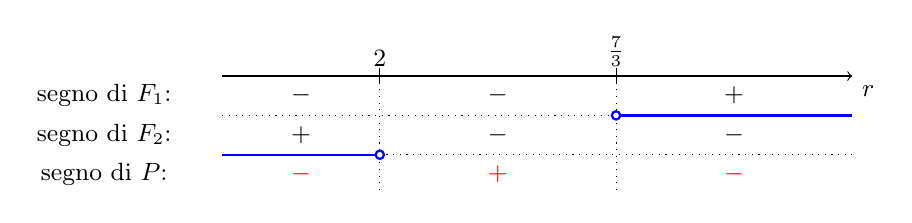
\begin{tikzpicture}[font=\small,x=10mm, y=10mm]

\draw[->] (0,0) -- (8,0) node [below right] () {$r$};

\foreach \x in {2,5}{
\draw(\x,3pt)--(\x,-3pt);
\begin{scope}[dotted]
\draw (\x,0) -- (\x,-1.5);
\draw (0,-.5) -- (5,-.5);
\draw (2,-1) -- (8,-1);
\end{scope}}

\node[above]  at (2,0) {$2$};
\node[above]  at (5,0) {$\frac{7}{3}$};

\begin{scope}[blue,thick]
\draw (5,-.5) -- (8,-.5);
\draw (0,-1) -- (2,-1);

\draw[fill=white] (5,-.5)circle (1.5pt);
\draw[fill=white] (2,-1)circle (1.5pt);
\end{scope}

\foreach \x in {-1.5}{
\node  at (\x,-.25) {segno di $F_1$:};
\node  at (\x,-.75) {segno di $F_2$:};
\node  at (\x,-1.25) {segno di $P$:};
}
\foreach \z in {1,3.5}{
\node  at (\z,-.25) {$-$};
}
\foreach \zi in {3.5, 6.5}{
\node  at (\zi,-.75) {$-$};
}

\node  at (6.5,-.25) {$+$};
\node  at (1,-.75) {$+$};

\begin{scope}[red]
\foreach \zii in {1, 6.5}{
\node  at (\zii,-1.25) {$-$};
}
\node  at (3.5,-1.25) {$+$};
\end{scope}
\end{tikzpicture}

\end{center}

Applicando poi la regola dei
segni otteniamo il segno del polinomio~$P=(3x-7)\cdot (2-x)$.

Ricordiamo che la disequazione che stiamo risolvendo~$(3x-7)\cdot(2-x)>0$
è verificata quando il polinomio~$P=(3x-7)\cdot (2-x)$ è
positivo, cioè nell'intervallo in cui abbiamo
ottenuto il segno ``$+$''. Possiamo
concludere~$\IS=\left\{x\in\insR\mid 2<x<\frac{7}{3}\right\}=(2\text{,~}\frac{7}{3})$.
 \end{esempio}

 \begin{esempio}
$(x-3)\cdot (2x-9)\cdot (4-5x)>0.$

Determiniamo il segno di ciascuno dei suoi tre fattori:

\[
F_{1}: x-3>0\:\Rightarrow\: x>3;\quad
F_{2}: 2x-9>0\:\Rightarrow\: x>\frac{9}{2};\quad
F_{3}: 4-5x>0\:\Rightarrow\: x<\frac{4}{5}.
\]

Costruiamo la tabella dei segni:
\begin{center}
 % (c) 2012 Dimitrios Vrettos - d.vrettos@gmail.com
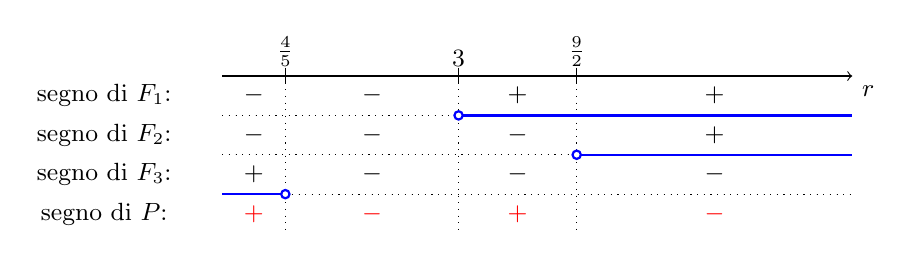
\begin{tikzpicture}[font=\small,x=10mm, y=10mm]

  \draw[->] (0,0) -- (8,0) node [below right] () {$r$};

  \foreach \x in {.8,3,4.5}{
    \draw(\x,3pt)--(\x,-3pt);

  \begin{scope}[dotted]
    \draw (\x,0) -- (\x,-2);
    \draw (0,-.5) -- (3,-.5);
    \draw (0,-1) -- (4.5,-1);
    \draw (.8,-1.5) -- (8,-1.5);
  \end{scope}}

  \node[above] at (.8,0) {$\frac{4}{5}$};
  \node[above]  at (3,0) {$3$};
  \node[above]  at (4.5,0) {$\frac{9}{2}$};

  \begin{scope}[blue,thick]
    \draw (3,-.5) -- (8,-.5);
    \draw (4.5,-1) -- (8,-1);
    \draw (0,-1.5) -- (.8,-1.5);

    \draw[fill=white] (3,-.5)circle (1.5pt);
    \draw[fill=white] (4.5,-1)circle (1.5pt);
    \draw[fill=white] (.8,-1.5)circle (1.5pt);
  \end{scope}

  \foreach \x in {-1.5}{
    \node  at (\x,-.25) {segno di $F_1$:};
    \node  at (\x,-.75) {segno di $F_2$:};
    \node  at (\x,-1.25) {segno di $F_3$:};
    \node  at (\x,-1.75) {segno di $P$:};
  }
  
  \foreach \z in {.4,1.9}
    \node  at (\z,-.25) {$-$};
  
  \foreach \zi in {.4,1.9, 3.75}
    \node  at (\zi,-.75) {$-$};

  \foreach \zii in {1.9, 3.75,6.25}
    \node  at (\zii,-1.25) {$-$};

  \foreach \ziii in {3.75,6.25}
    \node  at (\ziii,-.25) {$+$};

    \node  at (6.25,-.75) {$+$};
    \node  at (.4,-1.25) {$+$};

  \begin{scope}[red]
    \foreach \y in {-1.75}{
      \foreach \ziv in {.4,3.75}
	\node at (\ziv,\y) {$+$};
      \foreach \zv in {1.9,6.25}
	\node at (\zv,\y) {$-$};
      }
  \end{scope}
\end{tikzpicture}
\end{center}

La disequazione è verificata negli intervalli dove è presente il
segno ``$+$''.
\[\IS=\left\{x\in\insR\mid x<\frac{4}{5}\vee~3<x<\frac{9}{2}\right\}.\]
\end{esempio}

\begin{esempio}
 $4x^{3}+4x^{2}\le~1+x.$

La disequazione è di terzo grado. Trasportiamo al primo membro tutti i
monomi:
\[4x^{3}+4x^{2}-1-x\le~0.\]

Possiamo risolverla se riusciamo a scomporre in fattori di primo grado
il polinomio al primo membro:
\[4x^{3}+4x^{2}-1-x=4x^{2}(x+1)-(x+1)=(x+1)(4x^2-1)\:\Rightarrow\: (x+1)(2x-1)(2x+1)\le~0.\]

Studiamo ora il segno di ciascun fattore, tenendo conto che sono
richiesti anche i valori che annullano ogni singolo fattore (legge di
annullamento del prodotto):

\[ F_{1}:x+1\ge~0\:\Rightarrow\: x\ge -1;\quad F_{2}:2x-1\ge~0\:\Rightarrow\: x\ge \frac{1}{2};\quad F_{3}:2x+1\ge~0\:\Rightarrow\: x\ge -{\frac{1}{2}}.\]

Possiamo ora costruire la tabella dei segni.
Ricordiamo che la disequazione $P$ di partenza~$4x^{3}+4x^{2}\le~1+x$ è
verificata dove compare il segno~``$-$'':

\begin{center}
% (c) 2012 - 2013 Dimitrios Vrettos - d.vrettos@gmail.com
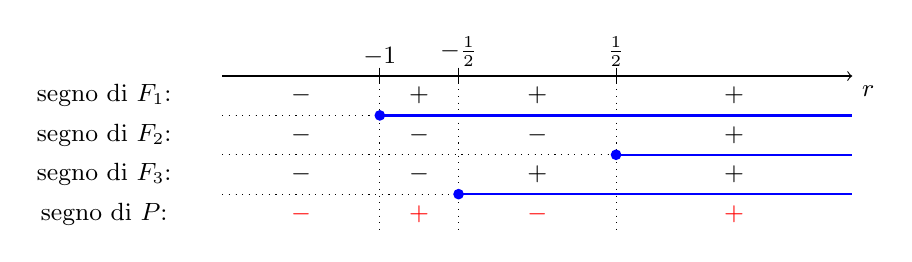
\begin{tikzpicture}[font=\small,x=10mm, y=10mm]

  \draw[->] (0,0) -- (8,0) node [below right] () {$r$};

  \foreach \x in {2,3,5}{
    \draw(\x,3pt)--(\x,-3pt);
    \begin{scope}[dotted]
      \draw (\x,0) -- (\x,-2);
      \draw (0,-.5) -- (2,-.5);
      \draw (0,-1) -- (5,-1);
      \draw (0,-1.5) -- (3,-1.5);
    \end{scope}}

  \node[above]  at (2,0) {$-1$};
  \node[above] at (3,0) {$-\frac{1}{2}$};
  \node[above]  at (5,0) {$\frac{1}{2}$};

  \begin{scope}[blue,thick]
    \draw (2,-.5) -- (8,-.5);
    \draw (5,-1) -- (8,-1);
    \draw (3,-1.5) -- (8,-1.5);

    \draw[fill=blue] (2,-.5)circle (1.5pt);
    \draw[fill=blue] (5,-1)circle (1.5pt);
    \draw[fill=blue] (3,-1.5)circle (1.5pt);
  \end{scope}

  \foreach \x in {-1.5}{
    \node  at (\x,-.25) {segno di $F_1$:};
    \node  at (\x,-.75) {segno di $F_2$:};
    \node  at (\x,-1.25) {segno di $F_3$:};
    \node  at (\x,-1.75) {segno di $P$:};}
  
  \foreach \z in {2.5,4,6.5}
    \node  at (\z,-.25) {$+$};
  
  \foreach \zi in {1,2.5, 4}
    \node  at (\zi,-.75) {$-$};
    
  \foreach \zii in {1,2.5}
    \node  at (\zii,-1.25) {$-$};
  

  \foreach \ziii in {4,6.5}
    \node  at (\ziii,-1.25) {$+$};

  \node  at (1,-.25) {$-$};
  \node  at (6.5,-.75) {$+$};


  \begin{scope}[red]
  \foreach \y in {-1.75}{
    \foreach \ziv in {2.5,6.5}
      \node at (\ziv,\y) {$+$};
    \foreach \zv in {1,4}
      \node at (\zv,\y) {$-$};
  }
  \end{scope}
\end{tikzpicture}

\end{center}
\[\IS=\left\{x\in \insR\mid x\le-1\text{ oppure }-\frac{1}{2}\le x\le\frac{1}{2}\right\}.\]
\end{esempio}
\end{exrig}

\begin{procedura}
 Determinare l'$\IS$ Di una disequazione polinomiale di grado
superiore al primo:

\begin{enumeratea}
 \item scrivere la disequazione nella forma~$P\leq0$, $P\geq~0$,
$P<0$, $P>0$;
\item scomporre in fattori irriducibili il polinomio $P$;
\item determinare il segno di ciascun fattore, ponendolo sempre maggiore
di zero, o maggiore uguale a zero a seconda della richiesta del
problema;
\item costruire la tabella dei segni, segnando con un punto ingrossato
gli zeri del polinomio;
\item determinare gli intervalli in cui il polinomio assume il segno
richiesto.
\end{enumeratea}
\end{procedura}

\ovalbox{\risolvii \ref{ese:21.44}, \ref{ese:21.45}, \ref{ese:21.46}, \ref{ese:21.47}, \ref{ese:21.48}, \ref{ese:21.49}, \ref{ese:21.50}, \ref{ese:21.51},
\ref{ese:21.52}, \ref{ese:21.53}}

\section{Disequazioni frazionarie}
Un'espressione contenente operazioni tra frazioni
algebriche ha come risultato una frazione algebrica. Con la condizione
di esistenza che il denominatore della frazione sia diverso da zero, la
ricerca del segno di una frazione algebrica viene effettuata con la
stessa procedura seguita per il prodotto di due o più fattori.

\begin{exrig}
 \begin{esempio}
 $P=\dfrac{3x-7}{2-x}\ge~0$.

 Poniamo innanzi tutto la~$\CE: 2-x\neq~0$
 cioè~$x\neq~2$ e procediamo studiando il segno del
numeratore $N$ e del denominatore $D$. Terremo conto della~$\CE$ ponendo il
denominatore $D$ semplicemente maggiore di zero e non maggiore uguale.
\[N\ge~0\:\Rightarrow\:~3x-7\ge~0\:\Rightarrow\: x\ge \frac{7}{3}\text{,}\]
\[D>0\:\Rightarrow\: 2-x>0\:\Rightarrow\: x<2.\]
\begin{center}
% (c) 2012 Dimitrios Vrettos - d.vrettos@gmail.com
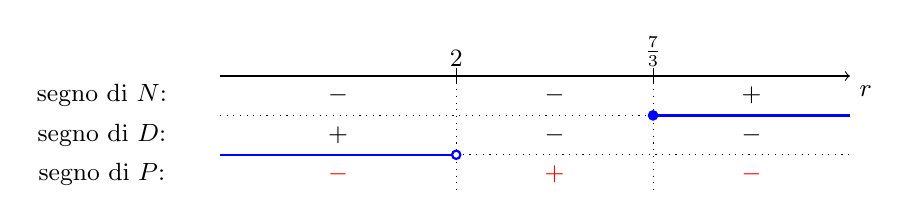
\begin{tikzpicture}[font=\small,x=10mm, y=10mm]

\draw[->] (0,0) -- (8,0) node [below right] () {$r$};

\foreach \x in {3,5.5}{
\draw(\x,3pt)--(\x,-3pt);
\begin{scope}[dotted]
\draw (\x,0) -- (\x,-1.5);
\draw (0,-.5) -- (5.5,-.5);
\draw (3,-1) -- (8,-1);
\end{scope}}

\node[above]  at (3,0) {$2$};
\node[above]  at (5.5,0) {$\frac{7}{3}$};

\begin{scope}[blue,thick]
\draw (5.5,-.5) -- (8,-.5);
\draw (3,-1) -- (0,-1);

\draw[fill=blue] (5.5,-.5)circle (1.5pt);
\draw[fill=white] (3,-1)circle (1.5pt);
\end{scope}

\foreach \x in {-1.5}{
\node  at (\x,-.25) {segno di $N$:};
\node  at (\x,-.75) {segno di $D$:};
\node  at (\x,-1.25) {segno di $P$:};
}
\foreach \z in {1.5,4.25}
\node  at (\z,-.25) {$-$};

\foreach \zi in {4.25,6.75}
\node  at (\zi,-.75) {$-$};

\node  at (6.75,-.25) {$+$};
\node  at (1.5,-.75) {$+$};

\begin{scope}[red]
\foreach \y in {-1.25}{
\foreach \ziv in {4.25}
	\node at (\ziv,\y) {$+$};
\foreach \zv in {1.5,6.75}
\node at (\zv,\y) {$-$};
}
\end{scope}
\end{tikzpicture}
\end{center}

Analogamente a quanto fatto per il prodotto, dalla tabella dei segni otteniamo
\[\IS=\left\{x\in \insR\mid 2<x\le \frac{7}{3}\right\}=\left(2\text{,~}\frac{7}{3}\right]\]
in cui vediamo già compresa la~$\CE$ che inizialmente avevamo posto.
 \end{esempio}
\end{exrig}

\begin{procedura}
 Procedura per determinare~$\IS$ di una disequazione frazionaria:

\begin{enumeratea}
\item applicare il primo principio e trasportare tutti i termini al primo membro;
 \item eseguire i calcoli dell'espressione al primo membro per arrivare a una disequazione nella forma:
 \subitem $\dfrac{N(x)}{D(x)}>0$ oppure~$\dfrac{N(x)}{D(x)}\ge~0$ oppure~$\dfrac{N(x)}{D(x)}<0$ oppure~$\dfrac{N(x)}{D(x)}\le~0$;
 \item studiare il segno del numeratore e del denominatore, ponendo~$N(x)>0$ (oppure~$N(x)\geq~0$ a secondo della richiesta) e~$D(x)>0$;
 \item costruire la tabella dei segni, segnando con un punto in grassetto gli zeri del numeratore;
 \item determinare gli intervalli in cui il polinomio assume il segno richiesto.
\end{enumeratea}
\end{procedura}

\begin{exrig}
 \begin{esempio}
 $\dfrac{x-1}{2x+2}+\dfrac{2x+1}{4x-2}>\dfrac{4x^{2}(2x+1)+1}{8x^{3}+8x^{2}-2x-2}.$

Trasportiamo tutti i termini al primo membro~$\dfrac{x-1}{2x+2}+\dfrac{2x+1}{4x-2}-\dfrac{4x^{2}(2x+1)+1}{8x^{3}+8x^{2}-2x-2}>0$.

Scomponiamo in fattori i denominatori, determiniamo il minimo comune
multiplo e sommiamo le frazioni per arrivare alla forma~$\frac{N(x)}{D(x)}>0$:

\begin{align}
&\frac{x-1}{2(x+1)}+\frac{2x+1}{2(2x-1)}-\frac{4x^{2}(2x+1)+1}{2(x+1)(2x-1)(2x+1)}>0 \notag\\
\Rightarrow & \frac{(x-1)(2x-1)(2x+1)+(2x+1)(2x+1)(x+1)-4x^{2}(2x+1)+1}{2(x+1)(2x-1)(2x+1)}>0 \notag\\
\Rightarrow & \frac{4x+1}{2(x+1)(2x-1)(2x+1)}>0. \label{eq:21.1}
\end{align}

Studiamo separatamente il segno di tutti i fattori che compaiono nella
frazione $F$, sia quelli al numeratore $N$ sia quelli al denominatore $D$ e
costruiamo la tabella dei segni:
 \[\begin{gathered}
 N>0\:\Rightarrow\: 4x+1>0\:\Rightarrow\: x>-{\frac{1}{4}}\text{,}\\
 D>0\:\Rightarrow\:\left\{\begin{array}{l}
			d_1:\: x+1>0\:\Rightarrow\: x>-1 \\
			d_2:\: 2x-1>0\:\Rightarrow\: x>\frac{1}{2}\\
			d_3:\: 2x+1>0\:\Rightarrow\: x>-{\frac{1}{2}}
		  \end{array}\right..
\end{gathered}\]
\begin{center}
% (c) 2012 Dimitrios Vrettos - d.vrettos@gmail.com
\begin{tikzpicture}[font=\small,x=10mm, y=10mm]

  \draw[->] (0,0) -- (8,0) node [below right] () {$r$};

  \foreach \x in {1.5,2.75,3.75,5.75}{
    \draw(\x,3pt)--(\x,-3pt);
    
    \begin{scope}[dotted]
      \draw (\x,0) -- (\x,-2.5);
      \draw (0,-.5) -- (3.75,-.5);
      \draw (0,-1) -- (1.5,-1);
      \draw (0,-1.5) -- (5.75,-1.5);
      \draw (0,-2) -- (2.75,-2);
    \end{scope}
  }

  \node[above]  at (1.5,0) {$-1$};
  \node[above] at (2.75,0) {$-\frac{1}{2}$};
  \node[above]  at (3.75,0) {$-\frac{1}{4}$};
  \node[above]  at (5.75,0) {$\frac{1}{2}$};

  \begin{scope}[blue,thick]
    \draw (3.75,-.5) -- (8,-.5);
    \draw (1.5,-1) -- (8,-1);
    \draw (5.75,-1.5) -- (8,-1.5);
    \draw (2.75,-2) -- (8,-2);

    \draw[fill=white] (3.75,-.5)circle (1.5pt);
    \draw[fill=white] (1.5,-1)circle (1.5pt);
    \draw[fill=white] (5.75,-1.5)circle (1.5pt);
    \draw[fill=white] (2.75,-2)circle (1.5pt);
  \end{scope}

  \foreach \x in {-1.5}{
    \node  at (\x,-.25) {segno di $N$:};
    \node(d1)  at (\x,-.75) {segno di $d_1$:};
    \node  at (\x,-1.25) {segno di $d_2$:};
    \node (d3) at (\x,-1.75) {segno di $d_3$:};
    \node  at (\x,-2.25) {segno di $F$ (\ref{eq:21.1}):};
    }

  \draw[decorate, decoration={brace, mirror}] let \p1=(d1.north west), \p2=(d3.south west) in(\p1 ) -- (\p2) node[midway, left=2pt] {$D:$};

  \foreach \z in {.75, 2.125,3.25}
    \node  at (\z,-.25) {$-$};

  \foreach \zi in {4.75, 6.875}
    \node  at (\zi,-.25) {$+$};

  \foreach \zii in {2.125,3.25,4.75, 6.875}
    \node  at (\zii,-.75) {$+$};

  \foreach \ziii in {.75,2.125,3.25,4.75}
    \node  at (\ziii,-1.25) {$-$};

  \foreach \ziv in {.75,2.125}
    \node at (\ziv,-1.75) {$-$};

  \foreach \zv in {3.25,4.75, 6.875}
    \node at (\zv,-1.75) {$+$};

  \node  at (.75,-.75) {$-$};
  \node  at (6.875,-1.25) {$+$};

  \begin{scope}[red]
    \foreach \y in {-2.25}{
      \foreach \ziv in {.75,3.25,6.875}
	\node at (\ziv,\y) {$+$};
      \foreach \zv in {2.125,4.75}
	\node at (\zv,\y) {$-$};
    }
  \end{scope}
\end{tikzpicture}

\end{center}
Non abbiamo posto le~$\CE$ in quanto già rispettate dalle disequazioni
del denominatore.
Prendiamo gli intervalli in cui il segno della frazione $F$ è positivo,
come richiesto dalla disequazione~\ref{eq:21.1}:
 \[\IS=\left\{x\in \insR\mid x<-1\vee -{\frac{1}{2}}<x<-{\frac{1}{4}}\vee x>\frac{1}{2}\right\}.\]
\end{esempio}

 \begin{esempio}
$\dfrac{x}{2}-\dfrac{2}{3}\cdot {\dfrac{2x-3}{x-1}}+\dfrac{10x-3}{6x-6}\le\dfrac{3}{2}\cdot {\dfrac{x^{2}+2}{3x-2}}+\dfrac{1}{3(x-1)(3x-2)}.$

Trasportiamo tutti i termini al primo membro:
\[\frac{x}{2}-\frac{2}{3}\cdot\frac{2x-3}{x-1}+\frac{10x-3}{6x-6}-\frac{3}{2}\cdot\frac{x^{2}+2}{3x-2}-\frac{1}{3(x-1)(3x-2)}\le~0.\]

Eseguiamo le operazioni per semplificare la frazione e ridurla alla
forma~$\frac{N(x)}{D(x)}\le~0$:

\begin{align}
  &\frac{x}{2}-\frac{4x-6}{3(x-1)}+\frac{10x-3}{6(x-1)}-\frac{3x^{2}+6}{2(3x-2)}-\frac{1}{3(x-1)(3x-2)}\le~0\notag\\
  \Rightarrow &\frac{3x(x-1)(3x-2)-2(4x-6)(3x-2)+(10x-3)(3x-2)-3(3x^{2}+6)(x-1)-2}{6(x-1)(3x-2)}\le~0\notag\\
  \Rightarrow &\frac{11x-2}{6(x-1)(3x-2)}\le~0. \label{eq:22.2}
\end{align}

Studiamo il segno di $F$, ovvero del suo numeratore $N$ e dei fattori del suo denominatore $D$:
 \[\begin{gathered}N\ge~0\:\Rightarrow\: 11x-2\ge 0\:\Rightarrow\: x\ge\frac{2}{11}\text{,}\\
		  D>0\:\Rightarrow\:\left\{\begin{array}{l}
			d_{1}>0\:\Rightarrow\: x-1>0\:\Rightarrow\: x>1\\
			d_{2}>0\:\Rightarrow\: 3x-2>0\:\Rightarrow\: x>\dfrac{2}{3}
			\end{array}\right.. \end{gathered}\]
\begin{center}
% (c) 2012 Dimitrios Vrettos - d.vrettos@gmail.com
\begin{tikzpicture}[font=\small,x=10mm, y=10mm]

\draw[->] (0,0) -- (8,0) node [below right] () {$r$};

\foreach \x in {1,3.72,5.56}{
\draw(\x,3pt)--(\x,-3pt);
\begin{scope}[dotted]
\draw (\x,0) -- (\x,-2);
\draw (0,-.5) -- (1,-.5);
\draw (0,-1) -- (5.56,-1);
\draw (0,-1.5) -- (3.72,-1.5);

\end{scope}}


\node[above] at (1,0) {$\frac{2}{11}$};
\node[above]  at (3.72,0) {$\frac{2}{3}$};
\node[above]  at (5.56,0) {$1$};

\begin{scope}[blue,thick]
\draw (1,-.5) -- (8,-.5);
\draw (5.56,-1) -- (8,-1);
\draw (3.72,-1.5) -- (8,-1.5);

\draw[fill=blue] (1,-.5)circle (1.5pt);
\draw[fill=white] (5.56,-1)circle (1.5pt);
\draw[fill=white] (3.72,-1.5)circle (1.5pt);
\end{scope}

\foreach \x in {-1.5}{
\node  at (\x,-.25) {segno di $N$:};
\node(d1)  at (\x,-.75) {segno di $d_1$:};
\node (d2) at (\x,-1.25) {segno di $d_2$:};
\node (d3) at (\x,-1.75) {segno di $F$ (\ref{eq:22.2}):};
}

 \draw[decorate, decoration={brace, mirror}]  let \p1=(d1.north west), \p2=(d2.south west) in(\p1 ) -- (\p2) node[midway, left=2pt] {$D:$};

\foreach \z in {2.36,4.64,6.78}
\node  at (\z,-.25) {$+$};

 \foreach \zi in {.5,2.36,4.64}
 \node  at (\zi,-.75) {$-$};

\foreach \zii in {.5,2.36}
 \node  at (\zii,-1.25) {$-$};

 \foreach \ziii in {4.64,6.78}
\node  at (\ziii,-1.25) {$+$};

\node  at (.5,-.25) {$-$};
\node  at (6.78,-.75) {$+$};

\begin{scope}[red]
\foreach \y in {-1.75}{
\foreach \ziv in {.5,4.64}
	\node at (\ziv,\y) {$-$};
\foreach \zv in {2.36,6.78}
\node at (\zv,\y) {$+$};
}
\end{scope}
\end{tikzpicture}

\end{center}
Non abbiamo posto le~$\CE$ in quanto già rispettate dalle disequazioni
del denominatore. Prendiamo gli intervalli in cui il segno della frazione $F$ è positivo o
nullo, come dalla disequazione~\ref{eq:22.2}:
\[\IS=\left\{x\in \insR\mid x\le\frac{2}{11}\vee \frac{2}{3}<x<1\right\}.\]
 \end{esempio}
\end{exrig}
\ovalbox{\risolvii \ref{ese:21.54}, \ref{ese:21.55}, \ref{ese:21.56}, \ref{ese:21.57}, \ref{ese:21.58}, \ref{ese:21.59}, \ref{ese:21.60}, \ref{ese:21.61}, \ref{ese:21.62}, \ref{ese:21.63}}

\vspazio\ovalbox{\ref{ese:21.64}, \ref{ese:21.65}, \ref{ese:21.66}, \ref{ese:21.67}, \ref{ese:21.68}, \ref{ese:21.69}}
\newpage
% (c) 2012-2014 - Dimitrios Vrettos d.vrettos@gmail.com
\section{Esercizi}
\subsection{Esercizi dei singoli paragrafi}
\subsubsection*{21.1 - Equazione lineare in due incognite}

\begin{esercizio}
 \label{ese:21.1}
Completa la tabella delle coppie di soluzioni dell'equazione~$x+2y-1=0$.

\begin{tabular*}{.9\textwidth}{@{\extracolsep{\fill}}*{10}{lccccccccc}}
\toprule
$x$ & & $-1$ & 0 & &$\frac{1}{2}$ & & & $\np{2,25}$ &\\
$y$ & 0 & & & $-1$ & & $\frac{3}{4}$ & 2 & & $\np{1,5}$\\
\bottomrule
\end{tabular*}
\end{esercizio}

\begin{esercizio}
 \label{ese:21.2}
Completa la tabella delle coppie di soluzioni dell'equazione~$3x-2y=5$.

\begin{tabular*}{.9\textwidth}{@{\extracolsep{\fill}}*{10}{lccccccccc}}
\toprule
$x$ & & 0 & 1 & & $\frac{1}{6}$ & & & $-\sqrt{2}$ & $\np{0,25}$\\
$y$ & 0 & & &$-1$ & & $\frac{3}{4}$ & $\sqrt{2}$ & & \\
\bottomrule
\end{tabular*}
\end{esercizio}

\begin{esercizio}
 \label{ese:21.3}
 Completa la tabella delle coppie di soluzioni dell'equazione~$3x-2\sqrt{2}\,y=0$.

 \begin{tabular*}{.9\textwidth}{@{\extracolsep{\fill}}*{8}{lccccccc}}
\toprule
$x$ & & 0 & & & $\frac{1}{6}$ & & $\sqrt{2}$ \\
$y$ & 0 & & 1 &$-1$ & & $\sqrt{2}$ & \\
\bottomrule
\end{tabular*}
\end{esercizio}

%%%%%%%%%%%%%%%%%%%%%%%%%%%%%%%%%%%%%%%%%%%%%%%%%%%%%%%%%%
\begin{esercizio}
 \label{ese:21.4}
Risolvi graficamente le seguenti equazioni in due incognite.
\begin{multicols}{2}
 \begin{enumeratea}
\spazielenx
\item $2x-2y+3=0$;
\item $-{\dfrac{1}{5}}x-\dfrac{5}{2}y+1=0$;
\item $-2y+3=0$;
\item $x+2y+\dfrac{7}{4}=0$.
\end{enumeratea}
\end{multicols}
\end{esercizio}

\begin{esercizio}
 \label{ese:21.5}
Risolvi graficamente le seguenti equazioni in due incognite.
\begin{multicols}{2}
 \begin{enumeratea}
\spazielenx
\item $-2x+4y-1=0$;
\item $2y+\dfrac{2}{3}x+6=0$;
\item $\sqrt{2}\,x+\sqrt{6}\,y=0$;
\item $\sqrt{3}\,y+\sqrt{6}=-x$.
 \end{enumeratea}
\end{multicols}
\end{esercizio}

\begin{esercizio}
 \label{ese:21.6}
 Stabilisci quali coppie appartengono all'Insieme Soluzione dell'equazione.
\TabPositions{4cm}
\begin{enumeratea}
\item $5x+7y-1=0$\tab$\left(-\frac{7}{5};0\right)$, $\left(-\frac{1}{5};-1\right)$, $\left(0;\frac{1}{7}\right)$, $\left(\frac{2}{5};-\frac{1}{7}\right)$;
\item $-x+\dfrac{3}{4}y-\dfrac{4}{3}=0$\tab$(0;-1)$, $\left(\frac{1}{12};\frac{7}{9}\right)$, $\left(-\frac{4}{3};0\right)$, $(-3;4)$;
\item $-x-y+\sqrt{2}=0$\tab$\left(\sqrt{2};0\right)$, $\left(0;-\sqrt{2}\right)$, $\left(1+\sqrt{2};-1\right)$, $\left(1;-1-\sqrt{2}\right)$.
\end{enumeratea}
\end{esercizio}

%%%%%%%%%%%%%%%%%%%%%%%%%%%%%%%%%%%%%%%%%%%%%%%%%%%%%%%%%%

\begin{esercizio}
 \label{ese:21.7}
Risolvi i seguenti sistemi con il metodo di sostituzione.
 \begin{multicols}{2}
 \begin{enumeratea}
  \item $\left\{\begin{array}{l}
     y=-2\\
     2x-y+2=0
    \end{array}\right.;$
  \item $\left\{\begin{array}{l}
	   y=-x+1\\
	   2x+3y+4=0
       \end{array}\right..$
 \end{enumeratea}
 \end{multicols}
\end{esercizio}

\begin{esercizio}[\Ast]
 \label{ese:21.8}
Risolvi i seguenti sistemi con il metodo di sostituzione.
 \begin{multicols}{2}
 \begin{enumeratea}
  \item $\left\{\begin{array}{l}
        x=1\\
        x+y=1
       \end{array}
\right.;$
\item $\left\{\begin{array}{l}
        y=x\\
        2x-y+2=0
       \end{array}\right.;$
\item $\left\{\begin{array}{l}
		2x+y=1\\
		2x-y=-1
	  \end{array}\right.;$
\item $\left\{\begin{array}{l}
	   2y=2\\
	   x+y=1
	\end{array}\right..$
 \end{enumeratea}
 \end{multicols}
\end{esercizio}
%\newpage
\begin{esercizio}[\Ast]
 \label{ese:21.9}
Risolvi i seguenti sistemi con il metodo di sostituzione.
 \begin{multicols}{2}
 \begin{enumeratea}
  \item $\left\{\begin{array}{l}3x-y=7\\x+2y=14\end{array}\right.;$
\item $\left\{\begin{array}{l}3x-2y=1\\4y-6x=-2\end{array}\right.;$
\item $\left\{\begin{array}{l}3x+y=2\\x+2y=-1\end{array}\right.;$
\item ${\longarray\left\{\begin{array}{l}x+4y-1=3\\
	\dfrac{x}{2}+\dfrac{y}{3}+1=-{\dfrac{x}{6}}-1
	\end{array}\right..}$
 \end{enumeratea}
 \end{multicols}
\end{esercizio}

\begin{esercizio}[\Ast]
 \label{ese:21.10}
Risolvi i seguenti sistemi con il metodo di sostituzione.
 \begin{multicols}{2}
 \begin{enumeratea}
  \item $\left\{\begin{array}{l}2x-3y=2\\6x-9y=6\end{array}\right.;$
\item $\left\{\begin{array}{l}x+2y=14\\3x-y=7\end{array}\right.;$
\item $\left\{\begin{array}{l}x+2y=1\\-2x-4y=2\end{array}\right.;$
\item $\left\{\genfrac{}{}{0pt}{0}{2x-y=3}{-6x+3y=-9}\right..$
 \end{enumeratea}
 \end{multicols}
\end{esercizio}

\begin{esercizio}[\Ast]
 \label{ese:21.11}
Risolvi i seguenti sistemi con il metodo di sostituzione.
 \begin{multicols}{2}
 \begin{enumeratea}
 \item $\longarray\left\{\begin{array}{l}\dfrac{x-4y}{3}=x-5y\\x-2=6y+4 \end{array}\right.;$
\item $\longarray\left\{\begin{array}{l}\dfrac{y^{2}-4x+2}{5}=\dfrac{2y^{2}-x}{10}-1\\x=-2y+8\end{array}\right.;$
\item $\longarray\left\{\begin{array}{l}3x-\dfrac{3}{4}(2y-1)=\dfrac{13}{4}(x+1)\\\dfrac{x+1}{4}-\dfrac{y}{2}=\dfrac{1+y}{2}-\dfrac{1}{4}\end{array}\right.;$
\item $\longarray\left\{\begin{array}{l}\dfrac{x}{3}-\dfrac{y}{2}=0\\\dfrac{y-x-1}{2}+x-y+1=\dfrac{1}{2}\end{array}\right..$
 \end{enumeratea}
 \end{multicols}
\end{esercizio}

\begin{esercizio}[\Ast]
 \label{ese:21.12}
Risolvi i seguenti sistemi con il metodo di sostituzione.
 \begin{multicols}{2}
 \begin{enumeratea}
  \item $\longarray\left\{\begin{array}{l}y-\dfrac{x}{3}+\dfrac{3}{4}=0\\\dfrac{2x+1}{1-x}+\dfrac{2+y}{y-1}=-1\end{array}\right.;$
\item $\longarray\left\{\begin{array}{l}x+y=2\\3\left(\dfrac{x}{6}+3y\right)=4\end{array}\right.;$
\item $\longarray\left\{\begin{array}{l}\dfrac{1}{2}y-\dfrac{1}{6}x=5-\dfrac{6x+10}{4}\\2(x-2)-3x=40-6\left(y-\dfrac{1}{3}\right)\end{array}\right.;$
\item $\longarray\left\{\begin{array}{l}2\dfrac{y}{3}+x+1=0\\\dfrac{y+1}{2}+\dfrac{x-1}{3}+1=0\end{array}\right..$
 \end{enumeratea}
 \end{multicols}
\end{esercizio}

\begin{esercizio}[\Ast]
 \label{ese:21.13}
Risolvi i seguenti sistemi con il metodo di sostituzione.

 \begin{enumeratea}
  \item $\longarray\left\{\begin{array}{l}(x-2)^{2}+y=(x+1)(x-y)+(3-y)(2-x)\\\dfrac{x}{4}-2y=2 \end{array}\right.;$
  \item $\left\{\begin{array}{l}x+y+1=0 \\x-y+k=0 \end{array}\right.;$
\item $\longarray\left\{\begin{array}{l}y-\dfrac{3-2x}{3}=\dfrac{x-y}{3}+1\\\dfrac{x+1}{2}+\dfrac{5}{4}=y+\dfrac{2-3x}{4}\end{array}\right.;$
\item $\left\{\begin{array}{l}x-2y-3=0\\kx+(k+1)y+1=0 \end{array}\right..$
 \end{enumeratea}

\end{esercizio}

\begin{esercizio}
 \label{ese:21.14}
 Risolvere il sistema che formalizza il problema~\ref{pr:22.1} a pagina \pageref{pr:22.1}:
\[\longarray\left\{\begin{array}{l}2x+\dfrac{1}{2}y=98
\\2x+3y=170 \end{array}\right.\]
e concludere il problema determinando l'area del rettangolo.
\end{esercizio}

\begin{esercizio}
 \label{ese:21.15}
Determinare due numeri reali~$x$ e~$y$ tali che il
triplo della loro somma sia uguale al doppio del primo aumentato di~10
e il doppio del primo sia uguale al prodotto del secondo con~5.
 \end{esercizio}

%%%%%%%%%%%%%%%%%%%%%%%%%%%%%%%%%%%%%%%%%%%%%%%%%%%%%%%%%%
\begin{esercizio}[\Ast]
 \label{ese:21.16}
Applica il metodo del confronto per risolvere i seguenti sistemi.
 \begin{multicols}{2}
 \begin{enumeratea}
 \item $\left\{\begin{array}{l}x+y=0\\-x+y=0\end{array}\right.;$
\item $\left\{\begin{array}{l}3x+y=5\\x+2y=0\end{array}\right.;$
\item $\left\{\begin{array}{l}x=2\\x+y=3\end{array}\right.;$
\item $\left\{\begin{array}{l}x=-1\\2x-y=1\end{array}\right..$
 \end{enumeratea}
 \end{multicols}
\end{esercizio}

\begin{esercizio}[\Ast]
 \label{ese:21.17}
Applica il metodo del confronto per risolvere i seguenti sistemi.
 \begin{multicols}{2}
 \begin{enumeratea}
 \item $\left\{\begin{array}{l}y=2x-1\\y=2x\end{array}\right.;$
\item $\left\{\begin{array}{l}x-2y=1\\2x-y=7\end{array}\right.;$
\item $\left\{\begin{array}{l}x+y=2\\-x-y=2\end{array}\right.;$
\item $\left\{\begin{array}{l}2x-y=4\\x-\dfrac{1}{2}y=2\end{array}\right..$
 \end{enumeratea}
 \end{multicols}
\end{esercizio}

\begin{esercizio}[\Ast]
 \label{ese:21.18}
Applica il metodo del confronto per risolvere i seguenti sistemi.
 \begin{multicols}{2}
 \begin{enumeratea}
\item $\left\{\begin{array}{l}y-\dfrac{3x-4}{2}=1-\dfrac{y}{4}\\2y-2x=-{\dfrac{4}{3}}\end{array}\right.;$
\item $\longarray\left\{\begin{array}{l}\dfrac{2}{3}x-y+\dfrac{1}{3}=0\\x-\dfrac{2}{3}y+\dfrac{1}{3}=0\end{array}\right.;$
\item $\left\{\begin{array}{l}\dfrac{1}{2}y-\dfrac{1}{6}x=5-\dfrac{6x+10}{8}\\8(x-2)+3x=40-6\left(y-\dfrac{1}{6}\right)\end{array}\right.;$
\item $\left\{\begin{array}{l}x=\dfrac{y-4}{3}+1\\y=\dfrac{x+3}{3}\end{array}\right.;$
\item $\left\{\begin{array}{l}x-y+k=0\\x+y=k-1\end{array}\right..$
 \end{enumeratea}
 \end{multicols}
\end{esercizio}

\begin{esercizio}
 \label{ese:21.19}
In un triangolo isoscele la somma della base con il doppio del lato
è~$168\unit{m}$ e la differenza tra la metà della base e~$1/13$ del lato è~$28\unit{m}$.
Indicata con~$x$ la misura della base e con~$y$ quella del lato,
risolvete con il metodo del confronto il sistema lineare che formalizza
il problema. Determinate l'area del triangolo.
 \end{esercizio}
\pagebreak
%%%%%%%%%%%%%%%%%%%%%%%%%%%%%%%%%%%%%%%%%%%%%%%%%%%%%%%%%%
 \begin{esercizio}[\Ast]
 \label{ese:21.20}
Risolvere i seguenti sistemi con il metodo di riduzione.

\begin{multicols}{2}
 \begin{enumeratea}
 \item $\left\{\begin{array}{l}x+y=0\\-x+y=0\end{array}\right.;$
 \item $\left\{\begin{array}{l}2x+y=1 \\2x-y=-1\end{array}\right.;$
 \item $\left\{\begin{array}{l}2x+y=1+y\\4x+y=2\end{array}\right.;$
 \item $\left\{\begin{array}{l}x+y=0\\x-y=-1\end{array}\right..$
\end{enumeratea}
\end{multicols}
\end{esercizio}

\begin{esercizio}[\Ast]
 \label{ese:21.21}
Risolvere i seguenti sistemi con il metodo di riduzione.
\begin{multicols}{2}
 \begin{enumeratea}
 \item $\left\{\begin{array}{l}x-y=0\\-2x+3y=1\end{array}\right.;$
 \item $\left\{\begin{array}{l}2x=3-x\\2x+y=3\end{array}\right.;$
 \item $\longarray\left\{\begin{array}{l}\dfrac{2}{3}x+\dfrac{2}{3}y=3\\\dfrac{3}{2}x-\dfrac{3}{2}y=2\end{array}\right.;$
 \item $\left\{\begin{array}{l}5y+2x=1 \\3x+2y+2=0\end{array}\right..$
\end{enumeratea}
\end{multicols}

\end{esercizio}

\begin{esercizio}[\Ast]
 \label{ese:21.22}
Risolvere i seguenti sistemi con il metodo di riduzione.

 \begin{enumeratea}
 \item $\left\{\begin{array}{l}-3x+y=2\\5x-2y=7\end{array}\right.;$
 \item $\longarray\left\{\begin{array}{l}2x=3-x\\2x+y=3\end{array}\right.;$
 \item $\longarray\left\{\begin{array}{l}\dfrac{4}{3}x-\dfrac{4y-x}{2}+\dfrac{35}{12}-\dfrac{x+y}{4}=0\\\dfrac{3(x+y)}{2}-\dfrac{1}{2}(5x-y)=\dfrac{1}{3}(11-4x+y)\end{array}\right.;$
 \item $\left\{\begin{array}{l}x+ay+a=0\\2x-ay+a=0\end{array}\right.;$
 \item $\left\{\begin{array}{l}2ax+2y-1=0\\ax+y=3\end{array}\right..$
\end{enumeratea}
\end{esercizio}

\begin{esercizio}
 \label{ese:21.23}
Il segmento~$AB$ misura~$80\unit{cm}$; il punto~$P$ lo divide in due parti tali che il quadruplo della
parte minore uguagli il triplo della differenza fra la maggiore e il
triplo della minore. Determinare~$\overline{AP}$ e~$\overline{PB}$ formalizzando
il problema con un sistema lineare che risolverete con il metodo di
riduzione.
\begin{center}
 % (c) 2012 Dimitrios Vrettos - d.vrettos@gmail.com
\begin{tikzpicture}[font=\small,x=10mm, y=10mm]
\draw (0,0) --(8,0);
\foreach \x in {0,8}{
\draw (\x,3pt) -- (\x,-3pt);
}
\node [below left] at (0,0) {$A$};
\node[below right]  at (8,0) {$B$};
\draw[fill=blue] (1.5,0) circle (1.5pt) node [below]  {$P$};

\end{tikzpicture}

\end{center}
\end{esercizio}

%%%%%%%%%%%%%%%%%%%%%%%%%%%%%%%%%%%%%%%%%%%%%%%%%%%%%%%%%%
\begin{esercizio}
 \label{ese:21.24}
Stabilire se il sistema è determinato:
\[\left\{\begin{array}{l}(x-1)(x+1)-3(x-2)=2(x-y+3)+x^{2}\\x(x+y-3)+y(4-x)=x^{2}-4x+y\end{array}\right..\]
\end{esercizio}

\begin{esercizio}
 \label{ese:21.25}
Verificare che il determinante della matrice del sistema è nullo:
\[\longarray\left\{\begin{array}{l}\dfrac{3}{2}x-\dfrac{7}{4}y=10^{5}\\6x-7y=5^{10}\end{array}\right..\]
\end{esercizio}

 %%%%%%%%%%%%%%%%%%%%%%%%%%%%%%%%%%%%%%%%%%%%%%%%%%%%%%%%%%
 \begin{esercizio}[\Ast]
 \label{ese:21.26}
Risolvere con la regola di Cramer i seguenti sistemi.
\begin{multicols}{2}
\begin{enumeratea}
\item $\left\{\begin{array}{l}x-3y=2\\x-2y=2\end{array}\right.;$
\item $\left\{\begin{array}{l}2x+2y=3\\3x-3y=2\end{array}\right.;$
\item $\left\{\begin{array}{l}5y+2x=1 \\3x+2y+2=0\end{array}\right.;$
\item $\left\{\begin{array}{l}5x+2y=-1 \\3x-2y=1\end{array}\right..$
\end{enumeratea}
\end{multicols}
\end{esercizio}

\begin{esercizio}[\Ast]
 \label{ese:21.27}
Risolvere con la regola di Cramer i seguenti sistemi.
\begin{multicols}{2}
\begin{enumeratea}
\item $\longarray\left\{\begin{array}{l}\dfrac{1}{2}y-\dfrac{2}{3}y=2\\\dfrac{1}{3}x+\dfrac{1}{2}y=1 \end{array}\right.;$
\item $\longarray\left\{\begin{array}{l}\dfrac{y}{5}-\dfrac{x}{2}=10\\\dfrac{x}{3}+\dfrac{y}{2}=5 \end{array}\right.;$
\item $\left\{\begin{array}{l}2(x-2y)+3x-2(y+1)=0\\x-2(x-3y)-5y=6(x-1) \end{array}\right.;$
\item $\longarray\left\{\begin{array}{l}4-2x=\dfrac{3}{2}(y-1)\\\dfrac{2x+3y}{2}=\dfrac{7+2x}{2}\end{array}\right..$
\end{enumeratea}
\end{multicols}
\end{esercizio}

\begin{esercizio}[\Ast]
 \label{ese:21.28}
Risolvere con la regola di Cramer i seguenti sistemi.
\begin{multicols}{2}
\begin{enumeratea}
\item $\left\{\begin{array}{l}3x+y=-3\\-2x+3y=+2\end{array}\right.;$
\item $\left\{\begin{array}{l}6x-2y=5\\x+\frac{1}{2}y=0\end{array}\right.;$
\item $\left\{\begin{array}{l}10x-20y=-11\\x+y-1=0\end{array}\right.;$
\item $\left\{\begin{array}{l}2x-3y+1=0\\4x+6y=0\end{array}\right..$
\end{enumeratea}
\end{multicols}
\end{esercizio}

\begin{esercizio}[\Ast]
 \label{ese:21.29}
Risolvere con la regola di Cramer i seguenti sistemi.
\begin{multicols}{2}
\begin{enumeratea}
\item $\left\{\begin{array}{l}x+2y=1\\2x+4y=1\end{array}\right.;$
\item $\left\{\begin{array}{l}3x+2y=4\\\frac{3}{2}x+y=2\end{array}\right.;$
\item $\left\{\begin{array}{l}ax+ay=3a^{2}\\x-2y=-3a\end{array}\right.;$
\item $\left\{\begin{array}{l}3x-2y=8k\\x-y=3k\end{array}\right..$
\end{enumeratea}
\end{multicols}
\end{esercizio}

\begin{esercizio}
 \label{ese:21.30}
 Risolvi col metodo di Cramer il sistema
\[\longarray\left\{\begin{array}{l}25x-3y=18\\\dfrac{3(y+6)}{5}=5x\end{array}\right..\]

Cosa osservi?
\end{esercizio}

%%%%%%%%%%%%%%%%%%%%%%%%%%%%%%%%%%%%%%%%%%%%%%%%%%%%%%%%%%
\begin{esercizio}
 \label{ese:21.31}
Per ciascuno dei seguenti sistemi stabilisci se è determinato,
indeterminato o impossibile.
\begin{multicols}{2}
\begin{enumeratea}
\item $\left\{\begin{array}{l}x-2y=3 \\4x-8y=12\end{array}\right.;$
\item $\left\{\begin{array}{l}x-2y=3 \\2x-4y=5\end{array}\right.;$
\item $\left\{\begin{array}{l}x-2y=3 \\2x-6y=12\end{array}\right.;$
\item $\longarray\left\{\begin{array}{l}\dfrac{1}{2}x-\dfrac{3}{2}y=-2\\\dfrac{5}{4}x-\dfrac{15}{4}y=-{\dfrac{5}{2}}\end{array}\right..$
\end{enumeratea}
\end{multicols}
\end{esercizio}

\begin{esercizio}
 \label{ese:21.32}
Per ciascuno dei seguenti sistemi stabilisci se è determinato,
indeterminato o impossibile.
\begin{multicols}{2}
\begin{enumeratea}
\item $\longarray\left\{\begin{array}{l}\dfrac{1}{7}x-\dfrac{4}{5}y=0\\\dfrac{5}{4}x-7y=\dfrac{19}{2}\end{array}\right.;$
\item $\left\{\begin{array}{l}2x+y=1 \\2x-y=-1\end{array}\right.;$
\item $\left\{\begin{array}{l}-40x+12y=-3\\17x-2y=100\end{array}\right.;$
\item $\left\{\begin{array}{l}x-y=3 \\-x+y=1 \end{array}\right..$
\end{enumeratea}
\end{multicols}
\end{esercizio}

\begin{esercizio}
 \label{ese:21.33}
Per ciascuno dei seguenti sistemi stabilisci se è determinato,
indeterminato o impossibile.
\begin{multicols}{2}
\begin{enumeratea}
\item $\longarray\left\{\begin{array}{l}-x+3y=-{\dfrac{8}{15}}\\5x-15y=\dfrac{2^{3}}{3}\end{array}\right.;$
\item $\longarray\left\{\begin{array}{l}\dfrac{x}{2}=-{\dfrac{y}{2}}+1\\x+y=2\end{array}\right..$
\end{enumeratea}
\end{multicols}
\end{esercizio}

\begin{esercizio}
 \label{ese:21.34}
La somma di due numeri reali è~16 e il doppio del
primo aumentato di~4 uguaglia la differenza tra~5 e il doppio del
secondo. Stabilisci, dopo aver formalizzato il problema con un sistema
lineare, se è possibile determinare i due numeri.
\end{esercizio}

\begin{esercizio}
 \label{ese:21.35}
Stabilisci per quale valore di~$a$ il sistema
$\left\{\begin{array}{l}ax+y=-2\\-3x+2y=0\end{array}\right.$ è
determinato. Se~$a=-{\frac{3}{2}}$ il sistema è indeterminato o
impossibile?
\end{esercizio}

\begin{esercizio}
 \label{ese:21.36}
Perché se~$a=\frac{1}{3}$ il sistema
$\left\{\begin{array}{l}x+ay=2a\\3x+y=2\end{array}\right.$ è
indeterminato?
\end{esercizio}

\begin{esercizio}
 \label{ese:21.37}
Per quale valore di~$k$ il sistema risulta impossibile?
\[\left\{\begin{array}{l}2x-3ky=2k\\x-ky=2k \end{array}\right.. \]
\end{esercizio}

\begin{esercizio}
 \label{ese:21.38}
Per quale valore di~$k$ il sistema risulta indeterminato?
\[\left\{\begin{array}{l}(k-2)x+3y=6 \\(k-1)x+4y=8 \end{array}\right..\]
\end{esercizio}

%%%%%%%%%%%%%%%%%%%%%%%%%%%%%%%%%%%%%%%%%%%%%%%%%%%%%%%%%%
\begin{esercizio}[\Ast]
 \label{ese:21.39}
Risolvi graficamente i sistemi; in base al disegno verifica se le rette
sono incidenti, parallele o coincidenti e quindi se il sistema è
determinato, impossibile o indeterminato.
\begin{multicols}{2}
\begin{enumeratea}
\item $\left\{\begin{array}{l}y=2x-1\\y=2x+1\end{array}\right.;$
\item $\left\{\begin{array}{l}y=2x-2\\y=3x+1\end{array}\right.;$
\item $\left\{\begin{array}{l}y=x-1 \\2y=2x-2 \end{array}\right.;$
\item $\left\{\begin{array}{l}2x-y=2 \\2y-x=2\end{array}\right..$
\end{enumeratea}
\end{multicols}
\end{esercizio}

\begin{esercizio}[\Ast]
 \label{ese:21.40}
Risolvi graficamente i sistemi; in base al disegno verifica se le rette
sono incidenti, parallele o coincidenti e quindi se il sistema è
determinato, impossibile o indeterminato.
\begin{multicols}{2}
\begin{enumeratea}
\item $\left\{\begin{array}{l}{3x+y=-3}\\{-2x+3y=-2}\end{array}\right.;$
\item $\left\{\begin{array}{l}x-3y=2\\x-2y=2\end{array}\right.;$
\item $\left\{\begin{array}{l}{3x+y=-3}\\{-2x+3y=+2}\end{array}\right.;$
\item $\left\{\begin{array}{l}2x=2-y\\2x-y=1\end{array}\right..$
\end{enumeratea}
\end{multicols}
\end{esercizio}

\begin{esercizio}[\Ast]
 \label{ese:21.41}
Risolvi graficamente i sistemi; in base al disegno verifica se le rette
sono incidenti, parallele o coincidenti e quindi se il sistema è
determinato, impossibile o indeterminato.
\begin{multicols}{3}
\begin{enumeratea}
\item $\left\{\begin{array}{l}5x+2y=-1 \\3x-2y=1 \end{array}\right.;$
\item $\left\{\begin{array}{l}2x=3-x\\2x+y=3\end{array}\right.;$
\item $\left\{\begin{array}{l}2x=2-y\\2x-y=1\end{array}\right..$
\end{enumeratea}
\end{multicols}
\end{esercizio}

\begin{esercizio}
 \label{ese:21.42}
Vero o falso?
\TabPositions{11cm}
 \begin{enumeratea}
\item Risolvere graficamente un sistema lineare significa trovare il punto di intersezione di due rette? \tab\boxV\quad\boxF
\item Un sistema lineare determinato ha una sola coppia soluzione?\tab\boxV\quad\boxF
\item Un sistema lineare è impossibile quando le rette che rappresentano le sue equazioni coincidono?\tab\boxV\quad\boxF
\end{enumeratea}
\end{esercizio}

\begin{esercizio}
 \label{ese:21.43}
Completa:

\begin{itemize*}
\item se~$r_{1}\cap r_{2}=r_{1}=r_{2}$ allora il sistema è\dotfill;
\item se~$r_{1}\cap r_{2}=P$ (punto singolo) allora il sistema è\dotfill;
\item se~$r_{1}\cap r_{2}=\emptyset $ allora il sistema è\dotfill
\end{itemize*}
\end{esercizio}

%%%%%%%%%%%%%%%%%%%%%%%%%%%%%%%%%%%%%%%%%%%%%%%%%%%%%%%%%%
\subsubsection*{21.3 - Sistemi frazionari o fratti}

\begin{esercizio}[\Ast]
 \label{ese:21.44}
Verifica l'insieme soluzione dei seguenti sistemi.
\begin{multicols}{2}
\begin{enumeratea}
\item $\longarray\left\{\begin{array}{l}\dfrac{4y+x}{5x}=1\\\dfrac{x+y}{2x-y}=2\end{array}\right.;$
\item $\longarray\left\{\begin{array}{l}y=\dfrac{4x-9}{12}\\{\dfrac{y+2}{y-1}+\dfrac{1+2x}{1-x}+1=0}\end{array}\right.;$
\item $\longarray\left\{\begin{array}{l}2+3\dfrac{y}{x}=\dfrac{1}{x}\\3\dfrac{x}{y}-1=\dfrac{-2}{y} \end{array}\right.;$
\item $\longarray\left\{\begin{array}{l}\dfrac{y}{2x-1}=-1\\2\dfrac{x}{y-1}=1\end{array}\right..$
\end{enumeratea}
\end{multicols}
\end{esercizio}

\begin{esercizio}[\Ast]
 \label{ese:21.45}
Verifica l'insieme soluzione dei seguenti sistemi.
\begin{multicols}{2}
\begin{enumeratea}
\item $\longarray\left\{\begin{array}{l}3\dfrac{x}{y}-\dfrac{7}{y}=1\\2\dfrac{y}{x}+\dfrac{5}{x}=1\end{array}\right.;$
\item $\longarray\left\{\begin{array}{l}2\dfrac{x}{3y}-\dfrac{1}{3y}=1\\\dfrac{3}{y+2x}=-1\end{array}\right.;$
\item $\longarray\left\{\begin{array}{l}\dfrac{x}{9y}=-{\dfrac{1}{2}}+\dfrac{1}{3y}\\9\dfrac{y}{2x}-1-\dfrac{3}{x}=0\end{array}\right.;$
\item $\longarray\left\{\begin{array}{l}\dfrac{x}{2-\dfrac{y}{2}-2}=1\\\dfrac{x-y}{x+\dfrac{3}{2}y-1}=1\end{array}\right..$
\end{enumeratea}
\end{multicols}
\end{esercizio}

\begin{esercizio}[\Ast]
 \label{ese:21.46}
Verifica l'insieme soluzione dei seguenti sistemi.
\begin{multicols}{2}
\begin{enumeratea}
\item $\longarray\left\{\begin{array}{l}\dfrac{\dfrac{x}{2}+\dfrac{2y}{3}-\dfrac{1}{6}}{x+y-2}=6\\x+y=1\end{array}\right.;$
\item $\longarray\left\{\begin{array}{l}\dfrac{x-2y}{4}=\dfrac{\dfrac{x-y}{2}+2x}{4}\\\dfrac{x}{\dfrac{y}{3}+1}=1\end{array}\right.;$
\item $\longarray\left\{\begin{array}{l}\dfrac{x+3y-1}{x-y}=\dfrac{1}{y-x} \\x=2y-10 \end{array}\right.;$
\item $\longarray\left\{\begin{array}{l}\dfrac{2}{x-2}-\dfrac{3}{y+3}=1\\\dfrac{5}{y+3}=\dfrac{6}{2-x}-4\end{array}\right..$
\end{enumeratea}
\end{multicols}
\end{esercizio}

\begin{esercizio}[\Ast]
 \label{ese:21.47}
Verifica l'insieme soluzione dei seguenti sistemi.

\begin{enumeratea}
\item $\longarray\left\{\begin{array}{l}y-\dfrac{x}{3}+\dfrac{3}{4}=0\\\dfrac{2x+1}{1-x}+\dfrac{2+y}{y-1}=-1\end{array}\right.;$
\item $\longarray\left\{\begin{array}{l}x+y=2\\y\left(\dfrac{x}{y}+3\right)=4\end{array}\right.;$
\item $\longarray\left\{\begin{array}{l}\dfrac{x}{3}-\dfrac{y}{2}=0\\\dfrac{y(y-x-1)}{y+1}+x-y+1=\dfrac{1}{2}\end{array}\right.;$
\item $\longarray\left\{\begin{array}{l}\dfrac{3x-7y+1}{4x^{2}-9y^{2}}=\dfrac{4}{18y^{2}-8x^{2}}\\\dfrac{4(1-3x)^{2}}{2}-y=\dfrac{(12x-5)(6x-y)}{4}+3xy+2\end{array}\right..$
\end{enumeratea}
\end{esercizio}

\begin{esercizio}[\Ast]
 \label{ese:21.48}
Verifica l'insieme soluzione dei seguenti sistemi.

\begin{enumeratea}
\item $\longarray\left\{\begin{array}{l}\dfrac{2x-3y}{x-2y}-\dfrac{3y-1}{x+5y}=\dfrac{2(x^{2}+2xy)-(3y-2)^{2}}{x^{2}+3xy-10y^{2}}\\x+y=-19\end{array}\right.;$
\item $\longarray\left\{\begin{array}{l}\dfrac{x-3}{x-3y+1}+\dfrac{xy-y}{x-3y-1}=\dfrac{x^{2}-3xy+x^{2}y-3xy^{2}+3y^{2}}{x^{2}+9y^{2}-6xy-1}\\\dfrac{x-3}{5y-1}-\dfrac{y-3}{1+5y}=\dfrac{x+5y^{2}-5xy+2}{1-25y^{2}}\end{array}\right.;$
\item $\longarray\left\{\begin{array}{l}\dfrac{x-2y}{x^{2}-xy-2y^{2}}-\dfrac{1}{y}=2\\\dfrac{4}{y}-\dfrac{5}{x+y}=-9\end{array}\right.;$
\item $\longarray\left\{\begin{array}{l}{2x-y-11=0}\\{\dfrac{y+1}{x-1}+\dfrac{3-y}{5x-5}-\dfrac{2}{3}=0}\end{array}\right..$
\end{enumeratea}
\end{esercizio}

\begin{esercizio}
 \label{ese:21.49}
Verifica l'insieme soluzione dei seguenti sistemi.
\begin{multicols}{2}
\begin{enumeratea}
\item $\longarray\left\{\begin{array}{l}{\dfrac{x+1}{x}=\dfrac{y+2}{y-2}}\\{\dfrac{3x-1}{3x-2}=\dfrac{1+y}{y-2}}\end{array}\right.;$
\item $\longarray\left\{\begin{array}{l}{\dfrac{2}{5x-y}=\dfrac{-3}{5y-x}}\\{\dfrac{1}{4x-3y}=\dfrac{2x+y-1}{3y-4x}}\end{array}\right.;$
\item $\longarray\left\{\begin{array}{l}{\dfrac{\sqrt{3}}{x-\sqrt{2}}+\dfrac{2\sqrt{2}}{y-\sqrt{3}}=0}\\{\dfrac{1}{x-\sqrt{3}}-\dfrac{\sqrt{6}}{2\left(y+2\sqrt{2}\right)}=0}\end{array}\right.;$
\item $\longarray\left\{\begin{array}{l}{\dfrac{x-y+1}{x+y-1}=2}\\{\dfrac{x+y+1}{x-y-1}=-2}\end{array}\right.;$
\item $\longarray\left\{\begin{array}{l}{\dfrac{2}{x-2}=\dfrac{3}{y-3}}\\{\dfrac{1}{y+3}=\dfrac{-1}{2-x}}\end{array}\right..$
\end{enumeratea}
\end{multicols}
\end{esercizio}

%%%%%%%%%%%%%%

\subsubsection*{21.4 - Sistemi letterali}

\begin{esercizio}[\Ast]
 \label{ese:21.50}
Risolvere e discutere il seguente sistema. Per quali valori di~$a$ la coppia soluzione è formata da
numeri reali positivi?
\[\left\{\begin{array}{l}{x+ay=2a}\\\dfrac{x}{2a}+y=\dfrac{3}{2}\end{array}\right..\]
\end{esercizio}


\begin{esercizio}
 \label{ese:21.51}
Perché se il seguente sistema è determinato la coppia soluzione è accettabile?
\[\left\{\begin{array}{l}3x-2y=0\\\dfrac{2x-y}{x+1}=\dfrac{1}{a}\end{array}\right..\]
\end{esercizio}


\begin{esercizio}
 \label{ese:21.52}
Nel seguente sistema è vero che la coppia soluzione è formata da numeri reali positivi se~$a>2$?
 \[\left\{\begin{array}{l}\dfrac{a-x}{a^{2}}+a+\dfrac{y-2a}{a+1}=-1\\2y=x\end{array}\right..\]
\end{esercizio}


\begin{esercizio}
 \label{ese:21.53}
Spiegate perché non esiste alcun valore di~$a$ per cui la
coppia~$(0;2)$ appartenga a~$\IS$ del sistema:
\[\left\{\begin{array}{l}3x-2y=0\\\dfrac{2x-y}{x+1}=\dfrac{1}{a}\end{array}\right..\]
\end{esercizio}

\begin{esercizio}[\Ast]
 \label{ese:21.54}
Nel seguente sistema determinate i valori da attribuire al
parametro~$a$ affinché la coppia soluzione accettabile sia formata da
numeri reali positivi.
\[\left\{\begin{array}{l}\dfrac{y}{x}-\dfrac{y-a}{3}=\dfrac{1-y}{3}\\a(x+2)+y=1\end{array}\right..\]
\end{esercizio}

\begin{esercizio}[\Ast]
 \label{ese:21.55}
Risolvere i seguenti sistemi.
\begin{multicols}{2}
 \begin{enumeratea}
 {\longarray
\item $\left\{\begin{array}{l}x+ay=2a\\\dfrac{x}{2a}+y=\dfrac{3}{2}\end{array}\right.;$
\item $\left\{\begin{array}{l}\dfrac{x^{3}-8}{x-2}=x^{2}-3x+y-2\\\dfrac{x^{2}-4xy+3y^{2}}{3y-x}=k\end{array}\right.;$
\item $\left\{\begin{array}{l}kx-y=2\\x+6ky=0\end{array}\right.;$
\item $\left\{\begin{array}{l}kx-8y=4\\2x-4ky=3\end{array}\right..$}
 \end{enumeratea}
\end{multicols}
\end{esercizio}

\begin{esercizio}[\Ast]
 \label{ese:21.56}
Risolvere i seguenti sistemi.
\begin{multicols}{2}
 \begin{enumeratea}
\item $\left\{\begin{array}{l}4x-k^{2}y=k\\kx-4ky=-3k\end{array}\right.;$
\item $\left\{\begin{array}{l}kx-4ky=-6\\kx-k^{2}y=0\end{array}\right.;$
\item $\left\{\begin{array}{l}(k-1)x+(1-k)y=0\\(2-2k)x+y=-1\end{array}\right..$
 \end{enumeratea}
\end{multicols}
\end{esercizio}

 \subsubsection*{21.5 - Sistemi lineari di tre equazioni in tre incognite}

\begin{esercizio}[\Ast]
 \label{ese:21.57}
 Determinare la terna di soluzione dei seguenti sistemi.
\begin{multicols}{2}
\begin{enumeratea}
\item $\left\{\begin{array}{l}x-2y+z=1 \\x-y=2 \\x+3y-2z=0 \end{array}\right.;$
\item $\left\{\begin{array}{l}x+y+z=4 \\x-3y+6z=1\\x-y-z=2 \end{array}\right.;$
\item $\left\{\begin{array}{l}x+2y-3z=6-3y\\2x-y+4z=x\\3x-z=y+2\end{array}\right.;$
\item $\left\{\begin{array}{l}2x-y+3z=1 \\x-2y+z=5\\x+2z=3 \end{array}\right.;$
\item $\left\{\begin{array}{l}x+2y-z=1 \\y-4z=0\\x-2y+z=2 \end{array}\right.;$
\item $\left\{\begin{array}{l}x-3y+6z=1 \\x+y+z=5 \\x+2z=3 \end{array}\right.;$
\end{enumeratea}
\end{multicols}
\end{esercizio}

\begin{esercizio}[\Ast]
 \label{ese:21.58}
 Determinare la terna di soluzione dei seguenti sistemi.
\begin{multicols}{3}
\begin{enumeratea}
\item $\left\{\begin{array}{l}x-4y+6z=2 \\x+4y-z=2\\x+3y-2z=2 \end{array}\right.;$
\item $\left\{\begin{array}{l}4x-y-2z=1 \\3x+2y-z=4\\x+y+2z=4 \end{array}\right.;$
\item $\left\{\begin{array}{l}x-3y=3 \\x+y+z=-1\\2x-z=0 \end{array}\right.;$
\item $\left\{\begin{array}{l}2x-y+3z=1 \\x-6y+8z=2\\3x-4y+8z=2 \end{array}\right.;$
\item $\left\{\begin{array}{l}4x-6y-7z=-1 \\x+y-z=1\\3x+2y+6z=1 \end{array}\right.;$
\item $\left\{\begin{array}{l}4x-3y+z=4\\x+4y-3z=2 \\y-7z=0 \end{array}\right..$
\end{enumeratea}
\end{multicols}
\end{esercizio}

\pagebreak
\begin{esercizio}[\Ast]
 \label{ese:21.59}
  Determinare la terna di soluzione dei seguenti sistemi.
\begin{multicols}{3}
\begin{enumeratea}
\item $\left\{\begin{array}{l}3x-6y+2z=1 \\x-4y+6z=5\\x-y+4z=10 \end{array}\right.;$
\item $\left\{\begin{array}{l}4x-y-7z=-12 \\x+3y+z=-4\\2x-y+6z=5 \end{array}\right.;$
\item $\left\{\begin{array}{l}2x+y-5z=2 \\x+y-7z=-2\\x+y+2z=1 \end{array}\right.;$
\item $\left\{\begin{array}{l}3x-y+z=-1\\x-y-z=3 \\x+y+2z=1 \end{array}\right.;$
\item $\left\{\begin{array}{l}x-4y+2z=7 \\-3x-2y+3z=0 \\x-2y+z=1 \end{array}\right.;$
\item $\left\{\begin{array}{l}-2x-2y+3z=4 \\2x-y+3z=0\\2x+y=1 \end{array}\right..$
\end{enumeratea}
\end{multicols}
\end{esercizio}


\begin{esercizio}
 \label{ese:21.60}
Quale condizione deve soddisfare il parametro~$a$ affinché il sistema seguente non sia privo di
significato? Determina la terna soluzione assegnando ad~$a$ il valore~2.
 \[\left\{\begin{array}{l}x+y+z=\dfrac{a^{2}+1}{a}\\ay-z=a^{2} \\y+ax=a+1+a^{2}z\end{array}\right..\]
\end{esercizio}

\begin{esercizio}
 \label{ese:21.61}
Determina il dominio del sistema e stabilisci se la terna soluzione è accettabile:
\[\longarray\left\{\begin{array}{l}\dfrac{5}{1-x}+\dfrac{3}{y+2}=\dfrac{2x}{xy-2+2x-y}\\
\dfrac{x+1-3(y-1)}{xyz}=\dfrac{1}{xy}-\dfrac{2}{yz}-\dfrac{3}{xz}\\
x+2y+z=0\end{array}\right..\]
\end{esercizio}

\begin{esercizio}
 \label{ese:21.62}
Verifica se il sistema è indeterminato:
\[\left\{\begin{array}{l}x+y=1 \\y-z=5
\\x+z+2=0 \end{array}\right..\]
\end{esercizio}

\begin{esercizio}
 \label{ese:21.63}
Determina il volume del parallelepipedo retto avente
per base un rettangolo, sapendo che le dimensioni della base e
l'altezza hanno come misura (in~$\unit{cm}$) i valori
di~$x$, $y$, $z$ ottenuti risolvendo il sistema:
\[\left\{\begin{array}{l}3x+1=2y+3z \\6x+y+2z=7
\\9(x-1)+3y+4z=0 \end{array}\right..\]
\end{esercizio}

%%%%%%%%%%%%%%%%%%%%%%%%%%%%%%%%%%%%%%%%%%%%

\subsubsection*{21.6 - Sistemi da risolvere con sostituzioni delle variabili}
\begin{esercizio}[\Ast]
 \label{ese:21.64}
 Risolvi i seguenti sistemi per mezzo di opportune sostituzioni delle variabili.

\begin{enumeratea}
\item $\longarray\left\{\begin{array}{l}\dfrac{1}{2x}+\dfrac{1}{y}=-4\\\dfrac{2}{3x}+\dfrac{2}{y}=1\end{array}\right.;$ \quad sostituire~$u=\dfrac{1}{x};v=\dfrac{1}{y}$.
\item $\left\{\begin{array}{l}x^{2}+y^{2}=13\\x^{2}-y^{2}=5 \end{array}\right.;$\quad sostituire~$u=x^{2};v=y^{2}$
\item $\longarray\left\{\begin{array}{l}\dfrac{1}{x+y}+\dfrac{2}{x-y}=1\\\dfrac{3}{x+y}-\dfrac{5}{x-y}=2\end{array}\right.;$\quad sostituire~$u=\dfrac{1}{x+y};v=\ldots$.
\end{enumeratea}
\end{esercizio}

\begin{esercizio}[\Ast]
 \label{ese:21.65}
 Risolvi i seguenti sistemi per mezzo di opportune sostituzioni delle variabili.
\begin{multicols}{2}
\begin{enumeratea}
{\longarray
\item $\left\{\begin{array}{l}\dfrac{5}{2x}-\dfrac{2}{y}=2\\\dfrac{1}{x}+\dfrac{2}{y}=1\end{array}\right.;$
\item $\left\{\begin{array}{l}\dfrac{1}{x}+\dfrac{2}{y}=3\\\dfrac{1}{x}+\dfrac{3}{y}=4\end{array}\right.;$
\item $\left\{\begin{array}{l}\dfrac{2}{x}+\dfrac{4}{y}=-3\\\dfrac{2}{x}-\dfrac{3}{y}=4 \end{array}\right.;$
\item $\left\{\begin{array}{l}\dfrac{1}{x+1}-\dfrac{2}{y-1}=2\\\dfrac{2}{x+1}-\dfrac{1}{y-1}=3\end{array}\right..$}
\end{enumeratea}
\end{multicols}
\end{esercizio}

\begin{esercizio}[\Ast]
 \label{ese:21.66}
 Risolvi i seguenti sistemi per mezzo di opportune sostituzioni delle variabili.
\begin{multicols}{2}
\begin{enumeratea}
\item $\longarray\left\{\begin{array}{l}\dfrac{1}{x}-\dfrac{3}{y}+\dfrac{2}{z}=3 \\\dfrac{2}{x}-\dfrac{3}{y}+\dfrac{2}{z}=4
\\\dfrac{2}{x}+\dfrac{4}{y}-\dfrac{1}{z}=-3\end{array}\right.;$
\item $\left\{\begin{array}{l}x^{3}+y^{3}=9 \\2x^{3}-y^{3}=-6 \end{array}\right.;$
\item $\left\{\begin{array}{l}x^{2}+y^{2}=-1\\x^{2}-3y^{2}=12\end{array}\right.;$
\item $\longarray\left\{\begin{array}{l}\dfrac{4}{x^{2}}-\dfrac{2}{y^{2}}-\dfrac{2}{z^{2}}=0\\\dfrac{1}{x^{2}}+\dfrac{1}{z^{2}}=2
\\\dfrac{2}{y^{2}}-\dfrac{2}{z^{2}}=0\end{array}\right..$
\end{enumeratea}
\end{multicols}
\end{esercizio}
%%%%%%%%%%%%%%%%%%%%%%%%%%%%%%%%%%%%%%%%%%%%%%%%%%%%%%%%%%%%

\subsection{Esercizi riepilogativi}
Gli esercizi indicati con (\croce) sono tratti da \emph{Matematica }~2, Dipartimento di
Matematica, ITIS V. Volterra, San Donà di Piave, Versione [11-12]~[S-A11], pg.~53; licenza CC, BY-NC-BD, per gentile concessione dei
professori che hanno reddatto il libro.% Il libro è scaricabile da \url{http://www.istitutovolterra.it/dipartimenti/matematica/dipmath/docs/M2_1112.pdf}

% il link http://www.istitutovolterra.it/dipartimenti/matematica/dipmath/docs/M2_1112.pdf non risulta essere più raggiungibile

\begin{esercizio}[\Ast]
 \label{ese:21.67}
 Risolvi i seguenti sistemi con più metodi ed eventualmente controlla
la soluzione graficamente.
\begin{multicols}{2}
\begin{enumeratea}
\item $\left\{\begin{array}{l}2x+y=1 \\2x-y=-1\end{array}\right.;$
\item $\left\{\begin{array}{l}2x=1+3y\\-y-2x=3\end{array}\right.;$
\item $\left\{\begin{array}{l}-x+2y=1 \\3x-y=3\end{array}\right.;$
\item $\left\{\begin{array}{l}5x-y=2\\2x+3y=-1 \end{array}\right..$
\end{enumeratea}
\end{multicols}
\end{esercizio}
%\newpage
\begin{esercizio}[\Ast]
 \label{ese:21.68}
 Risolvi i seguenti sistemi con più metodi ed eventualmente controlla
la soluzione graficamente.
\begin{multicols}{2}
\begin{enumeratea}
\item $\left\{\begin{array}{l}x+2y=3 \\3x-y=2\end{array}\right.;$
\item $\left\{\begin{array}{l}2x-y=1 \\x+2y=2\end{array}\right.;$
\item $\left\{\begin{array}{l}5x+3y=2 \\3x-2y=1\end{array}\right.;$
\item $\left\{\begin{array}{l}7x-2y=4\\8x-6y=9 \end{array}\right..$
\end{enumeratea}
\end{multicols}
\end{esercizio}

\begin{esercizio}[\Ast]
 \label{ese:21.69}
 Risolvi i seguenti sistemi con più metodi ed eventualmente controlla
la soluzione graficamente.
\begin{multicols}{2}
\begin{enumeratea}
\item $\left\{\begin{array}{l}3x-2y=4 \\2x+3y=5\end{array}\right.;$
\item $\left\{\begin{array}{l}3x-y=7 \\x-2y=5 \end{array}\right.;$
\item $\left\{\begin{array}{l}3x-2y=2\\2y-2x=-{\frac{4}{3}} \end{array}\right.;$
\item $\left\{\begin{array}{l}5x-2x=7\\-x-2y=-{\frac{1}{2}} \end{array}\right..$
\end{enumeratea}
\end{multicols}
\end{esercizio}

\begin{esercizio}[\Ast]
 \label{ese:21.70}
 Risolvi i seguenti sistemi con più metodi ed eventualmente controlla
la soluzione graficamente.
\begin{multicols}{2}
\begin{enumeratea}
{\longarray
\item $\left\{\begin{array}{l}\dfrac{2}{3}x-2y=-{\dfrac{1}{6}}\\-y-\dfrac{2}{3}y=\dfrac{3}{2} \end{array}\right.;$
\item $\left\{\begin{array}{l}\dfrac{1}{3}x-\dfrac{3}{2}y+1=0\\9y-2x-6=0 \end{array}\right.;$
\item $\left\{\begin{array}{l}-{\dfrac{1}{3}}x+\dfrac{3}{2}y-1=0\\3x-\dfrac{1}{5}y+\dfrac{3}{2}=0 \end{array}\right.;$
\item $\left\{\begin{array}{l}-{\dfrac{2}{3}}y+3x=y\\x-\dfrac{1}{2}y+3=0 \end{array}\right..$}
\end{enumeratea}
\end{multicols}
\end{esercizio}

\begin{esercizio}[\Ast]
 \label{ese:21.71}
 Risolvi i seguenti sistemi con più metodi ed eventualmente controlla
la soluzione graficamente.
\begin{multicols}{2}
\begin{enumeratea}
\item $\longarray\left\{\begin{array}{l}5y+\dfrac{3}{2}x=-2\\3x+10y-3=0 \end{array}\right.;$
\item $\left\{\begin{array}{l}{2x+y=0}\\{x-2y=-5}\end{array}\right.;$
\item $\longarray\left\{\begin{array}{l}\dfrac{1}{2}x-3y=\dfrac{1}{2}\\3(y-2)+x=0 \end{array}\right.;$
\item $\left\{\begin{array}{l}{x+y=-1}\\{x-y=5}\end{array}\right..$
\end{enumeratea}
\end{multicols}
\end{esercizio}

\begin{esercizio}[\Ast]
 \label{ese:21.72}
 Risolvi i seguenti sistemi con più metodi ed eventualmente controlla
la soluzione graficamente.
\begin{multicols}{2}
\begin{enumeratea}
\item $\left\{\begin{array}{l}{2x+2y=6}\\{x-2y=-3}\end{array}\right.;$
\item $\left\{\begin{array}{l}{\dfrac{1}{3}x+3y+2=0}\\{2x+\dfrac{1}{2}y=\dfrac{11}{2}}\end{array}\right.;$
\item $\left\{\begin{array}{l}{2x-y=3}\\{x-2y=0}\end{array}\right.;$
\item $\left\{\begin{array}{l}{\dfrac{1}{2}x+\dfrac{1}{2}y=1}\\{\dfrac{2}{3}x+\dfrac{1}{3}y=1}\end{array}\right..$
\end{enumeratea}
\end{multicols}
\end{esercizio}
%\newpage
\begin{esercizio}[\Ast]
 \label{ese:21.73}
 Risolvi i seguenti sistemi con più metodi ed eventualmente controlla
la soluzione graficamente.
\begin{multicols}{2}
\begin{enumeratea}
 {\longarray
\item $\left\{\begin{array}{l}{2x-y=0}\\{4x+\dfrac{1}{2}y=\dfrac{5}{2}}\end{array}\right.;$
\item $\left\{\begin{array}{l}{2x+\dfrac{1}{2}y=-\dfrac{3}{10}}\\{-25x+5y=6}\end{array}\right.;$
\item $\left\{\begin{array}{l}{2x+y-3=0}\\{4x+2y+6=0}\end{array}\right.;$
\item $\left\{\begin{array}{l}{2x-y=-1}\\{x+\dfrac{1}{2}y=-{\dfrac{1}{2}}}\end{array}\right..$}
\end{enumeratea}
\end{multicols}
\end{esercizio}

\begin{esercizio}[\Ast]
\label{ese:21.74}
Risolvi i seguenti sistemi con più metodi ed eventualmente controlla
la soluzione graficamente.
\begin{multicols}{2}
\begin{enumeratea}
 {\longarray
\item $\left\{\begin{array}{l}{\dfrac{1}{2}x-\dfrac{1}{3}y=1}\\{3x-2y=3}\end{array}\right.;$
\item $\left\{\begin{array}{l}{10x-5y=26}\\{x+5y=-\dfrac{42}{5}}\end{array}\right.;$
\item $\left\{\begin{array}{l}\dfrac{1}{2}(x-3)-y=\dfrac{3}{2}(y-1)\\\dfrac{3}{2}(y-2)+x=6\left(x+\dfrac{1}{3}\right)\end{array}\right.;$
\item $\left\{\begin{array}{l}\dfrac{x+4y}{6}-3=0\\\dfrac{x}{2}-\dfrac{y}{4}=0\end{array}\right..$}
\end{enumeratea}
\end{multicols}
\end{esercizio}

\begin{esercizio}[\Ast]
 \label{ese:21.75}
 Risolvi i seguenti sistemi con più metodi ed eventualmente controlla
la soluzione graficamente.

\begin{enumeratea}
 {\longarray
\item $\left\{\begin{array}{l}3(x-4)=-{\dfrac{4y}{5}}\\7(x+y)+8\left(x-\dfrac{3y}{8}-2\right)=0\end{array}\right.;$
\item $\left\{\begin{array}{l}\dfrac{2}{5}(y-x-1)=\dfrac{y-x}{3}-\dfrac{2}{5}\\(x-y)^{2}-x(x-2y)=x+y(y-1)\end{array}\right.;$
\item $\left\{\begin{array}{l}2x-3(x-y)=-1+3y\\\dfrac{1}{2}x+\dfrac{1}{3}y=-{\dfrac{1}{6}}\end{array}\right.;$
\item $\left\{\begin{array}{l}(y+2)(y-3)-(y-2)^{2}+(x+1)^{2}=(x+3)(x-3)-\dfrac{1}{2}\\\left(y-\dfrac{1}{2}\right)\left(y+\dfrac{1}{4}\right)-(y-1)^{2}+2x+3=\dfrac{3}{4}\end{array}\right..$}
\end{enumeratea}
\end{esercizio}
%\newpage
\begin{esercizio}[\Ast]
 \label{ese:21.76}
 Risolvi i seguenti sistemi con più metodi ed eventualmente controlla
la soluzione graficamente.
\begin{multicols}{2}
\begin{enumeratea}
 {\longarray
\item $\left\{\begin{array}{l}\dfrac{\dfrac{x}{2}-y+5}{\dfrac{4}{3}-\dfrac{5}{6}}=x-\dfrac{\dfrac{x}{2}-\dfrac{y}{3}}{2}\\-x-\dfrac{\dfrac{y}{3}-x}{2}=1\end{array}\right.;$
\item $\left\{\begin{array}{l}x^{2}+\dfrac{y}{4}-3x=\dfrac{(2x+1)^{2}}{4}-\dfrac{y}{2}\\(y-1)^{2}=-8x+y^{2}\end{array}\right.;$
\item $\left\{\begin{array}{l}\dfrac{\dfrac{x+1}{2}-y}{2}=y-20x\\x-\dfrac{y}{4}=\dfrac{x-y}{6}\end{array}\right.;$
\item $\left\{\begin{array}{l}\dfrac{4y-\dfrac{5}{2}x+\dfrac{3}{2}}{\dfrac{5}{6}}=x-2y\\x=3y\end{array}\right..$}
\end{enumeratea}
\end{multicols}
\end{esercizio}

%%%%%%%%%%%%%%%%%%%%%%%%%%%%%%%%%%%%%%%%%%%%%%%%%%%%%%%%%%%%%%%%%%%%%%%%%%
\begin{multicols}{2}
\begin{esercizio}
 \label{ese:21.77}
Determina due numeri sapendo che la loro somma è~37 e la loro
differenza è~5.
\end{esercizio}

\begin{esercizio}[\Ast]
 \label{ese:21.78}
Il doppio della somma di due numeri è uguale al secondo numero aumentato
del triplo del primo, inoltre aumentando il primo numero di~12 si
ottiene il doppio del secondo diminuito di~6.
\end{esercizio}

\begin{esercizio}[\Ast]
 \label{ese:21.79}
Determina tre numeri la cui somma è~81. Il secondo supera il primo
di~3. Il terzo numero è dato dalla somma dei primi due.
\end{esercizio}

\begin{esercizio}[\Ast]
 \label{ese:21.80}
Determina due numeri sapendo che la loro somma è pari al doppio del minore aumentato di~$1/4$
del maggiore, mentre la loro differenza è uguale a~$9$.
\end{esercizio}

\begin{esercizio}[\Ast]
 \label{ese:21.81}
Determina due numeri la cui somma è~57 e di cui si sa che il doppio del più grande
diminuito della metà del più piccolo è~49.
\end{esercizio}

\begin{esercizio}[\Ast]
 \label{ese:21.82}
Determina tre lati sapendo che il triplo del primo lato è
uguale al doppio del secondo aumentato di~$10\unit{m}$; la differenza tra il
doppio del terzo lato e il doppio del secondo lato è uguale al primo
lato aumentato di~12; la somma dei primi due lati è uguale al terzo
lato.
\end{esercizio}

\begin{esercizio}[\Ast]
 \label{ese:21.83}
Determina un numero di due cifre sapendo che la cifra delle decine
è il doppio di quella delle unità e scambiando le due cifre si
ottiene un numero più piccolo di~27 del precedente.
\end{esercizio}

\begin{esercizio}[\Ast]
 \label{ese:21.84}
Determina il numero intero di due
cifre di cui la cifra delle decine supera di~2 la cifra delle unità e
la somma delle cifre è~12.
\end{esercizio}

\begin{esercizio}[\croce]
 \label{ese:21.85}
Determina due numeri naturali il cui quoziente è~5 e la cui
differenza è~12.
\end{esercizio}

\begin{esercizio}[\Ast, \croce]
 \label{ese:21.86}
Determinare un numero naturale di due cifre sapendo che la loro somma
è~12 e che, invertendole, si ottiene un numero che supera di~6 la
metà di quello iniziale.
\end{esercizio}

\begin{esercizio}[\croce]
 \label{ese:21.87}
Determinare la frazione che diventa uguale a~$5/6$ aumentando i suoi
termini di~2 e diventa~$1/2$ se i suoi termini diminuiscono di~2.
\end{esercizio}

\begin{esercizio}[\Ast, \croce]
 \label{ese:21.88}
La somma delle età di due coniugi è~65 anni; un settimo
dell'età del marito è uguale ad un sesto
dell'età della moglie. Determinare le età dei
coniugi.
\end{esercizio}

\begin{esercizio}[\Ast, \croce]
 \label{ese:21.89}
Un numero naturale diviso per~3 dà un certo quoziente e resto~1. Un
altro numero naturale, diviso per~5, dà lo stesso quoziente e resto~3.
Sapendo che i due numeri hanno per somma~188, determinali e calcola
il quoziente.
\end{esercizio}

\begin{esercizio}[\Ast]
 \label{ese:21.90}
Giulio e Giulia hanno svuotato i loro
salvadanai per comparsi una bici. Nel negozio c'è
una bella bici che piace a entrambi e costa \officialeuro~$180$, ma nessuno dei
due ha i soldi sufficienti per comprarla. Giulio dice:
<<Se mi dai la metà dei tuoi soldi compro io la
bici>>. Giulia ribatte: <<se mi dai la terza
parte dei tuoi soldi la bici la compro io>>. Quanti soldi
hanno rispettivamente Giulio e Giulia?
\end{esercizio}

\begin{esercizio}
 \label{ese:21.91}
A una recita scolastica per beneficenza vengono incassati
\officialeuro~$216$ per un totale di~102 biglietti venduti. I ragazzi della
scuola pagano \officialeuro~$1$, i ragazzi che non sono di quella scuola
pagano \officialeuro~$\np{1,5}$ e gli adulti pagano \officialeuro~$3$. Quanti sono i
ragazzi della scuola che hanno assistito alla recita?
\end{esercizio}


\begin{esercizio}
 \label{ese:21.92}
Da un cartone quadrato di lato~$12\unit{cm}$, si taglia prima una scriscia
parallela a un lato e di spessore non noto, poi si taglia dal lato
adiacente una striscia parallela al lato spessa~$2\unit{cm}$ in più rispetto
alla striscia precedente. Sapendo che il perimetro del rettangolo
rimasto è~$\np[cm]{33,6}$, calcola l'area del rettangolo rimasto.
\end{esercizio}

\begin{esercizio}[\Ast]
 \label{ese:21.93}
Al bar per pagare~4 caffè e~2 cornetti si spendono \officialeuro~$\np{4,60}$, per pagare~6 caffè
e~3 cornetti si spendono \officialeuro~$\np{6,90}$. \`E possibile
determinare il prezzo del caffè e quello del cornetto?
\end{esercizio}

\begin{esercizio}[\Ast]
 \label{ese:21.94}
 Al bar, Mario offre la colazione agli amici perché è il suo
compleanno: per~4 caffè e~2 cornetti paga \officialeuro~$\np{4,60}$. Subito dopo
arrivano altri tre amici che prendono un caffè e un cornetto
ciascuno, e questa volta Mario paga \officialeuro~$\np{4,80}$. Quanto costa un caffè e
quanto un cornetto?
\end{esercizio}

\begin{esercizio}[\Ast]
 \label{ese:21.95}
Un cicloturista percorre~$218\unit{km}$ in tre giorni. Il secondo giorno percorre
il~$20\%$ in più del primo giorno. Il terzo giorno percorre~$14\unit{km}$ in
più del secondo giorno. Qual è stata la lunghezza delle tre tappe?
\end{esercizio}

\begin{esercizio}[\Ast]
 \label{ese:21.96}
In un parcheggio ci sono moto e auto. In tutto si contano~43 mezzi e~140
ruote. Quante sono le auto e quante le moto?
\end{esercizio}

\begin{esercizio}
 \label{ese:21.97}
Luisa e Marisa sono due sorelle. Marisa, la più grande, è nata~3 anni
prima della sorella e la somma delle loro età è~59. Qual è
l'età delle due sorelle?
\end{esercizio}

\begin{esercizio}
 \label{ese:21.98}
Mario e Lucia hanno messo da parte del denaro. Lucia ha \officialeuro~5
in più di Mario. Complessivamente potrebbero comprare
schede prepagate per i cellulari per \officialeuro~$45$. Quanto possiede Mario e quanto
Lucia?
\end{esercizio}

\begin{esercizio}
 \label{ese:21.99}
Una macchina per ghiaccio produce~10 cubetti di ghiaccio al minuto, mentre
una seconda macchina ne produce~7 al minuto. Sapendo
che in tutto sono stati prodotti~304 cubetti e che complessivamente le
macchine hanno lavorato per~22 minuti, quanti cubetti ha prodotto la
prima macchina e quanti ne ha prodotti la seconda?
\end{esercizio}

\begin{esercizio}[\Ast]
 \label{ese:21.100}
In un parcheggio ci sono automobili, camion e moto per un totale di~62 mezzi.
Le auto hanno~4 ruote, i camion ne hanno~6 e le moto ne hanno~2.
In totale le ruote sono~264. Il numero delle ruote delle auto è uguale
al numero delle ruote dei camion. Determina quante auto, quanti camion
e quante moto ci sono nel parcheggio.
\end{esercizio}

\begin{esercizio}
 \label{ese:21.101}
 Un vasetto di marmellata pesa~$780\unit{g}$. Quando nel vasetto rimane
metà marmellata, il vasetto pesa~$420\unit{g}$. Quanto pesa il vasetto vuoto?
\end{esercizio}


\begin{esercizio}[\Ast]
 \label{ese:21.102}
Una gelateria prepara per la giornata di Ferragosto~$30\unit{kg}$ di
gelato. Vende i coni da due palline a \officialeuro~$\np{1,50}$ e i coni da tre
palline a \officialeuro~$\np{2,00}$. Si sa che da~$2\unit{kg}$ di gelato si fanno~25
palline di gelato. A fine giornata ha venduto tutto il gelato e ha
incassato \officialeuro~$\np{272,50}$. Quanti coni da due palline ha venduto?
\end{esercizio}

\begin{esercizio}[Prove Invalsi~2004-2005]
 \label{ese:21.103}
Marco e Luca sono fratelli. La somma delle loro età è~23
anni. Il doppio dell'età di Luca è uguale alla
differenza tra l'età del loro padre e il triplo
dell'età di Marco. Quando Luca è nato, il padre
aveva~43 anni. Determina l'età di Marco e di Luca.
\end{esercizio}


\begin{esercizio}[Giochi d'autunno~2010, Centro Pristem]
 \label{ese:21.104}
Oggi Angelo ha un quarto dell'età di sua
madre. Quando avrà~18 anni, sua madre avrà il triplo della sua
età. Quanti anni hanno attualmente i due?
\end{esercizio}


\begin{esercizio}[Giochi di Archimede, 2008]
 \label{ese:21.105}
 Pietro e Paolo festeggiano il loro onomastico in pizzeria con i
loro amici. Alla fine della cena il conto viene diviso in parti uguali
tra tutti i presenti e ciascuno dovrebbe pagare \officialeuro~$12$. Con grande
generosità però gli amici decidono di offrire la cena a Pietro e
Paolo; il conto viene così nuovamente diviso in parti uguali tra gli amici
di Pietro e Paolo (cioè tutti i presenti esclusi Pietro e Paolo) e
ciascuno di loro paga \officialeuro~$16$. Quanti sono gli amici di Pietro e Paolo?
\end{esercizio}


\begin{esercizio}[\Ast]
 \label{ese:21.106}
 Al bar degli studenti caffè e cornetto costano
\officialeuro~$\np{1,50}$; cornetto e succo di frutta costano \officialeuro~$\np{1,80}$,
caffè e succo di frutta costano \officialeuro~$\np{1,70}$. Quanto costano in
tutto~7 caffè,~5 cornetti e~3 succhi di frutta?
\end{esercizio}

\begin{esercizio}[\croce]
 \label{ese:21.107}
Un negozio ha venduto scatole contenenti~6 fazzoletti ciascuna
ed altre contenenti~12 fazzoletti ciascuna, per un totale di~156
fazzoletti. Il numero delle confezioni da~12 ha superato di~1 la metà
di quello delle confezioni da~6. Quante confezioni di ogni tipo si sono
vendute?
\end{esercizio}


\begin{esercizio}[\Ast, \croce]
 \label{ese:21.108}
Nella città di Nonfumo gli unici negozi sono tabaccherie e
latterie. L'anno scorso le tabaccherie erano i~$2/3$
delle latterie; quest'anno due tabaccherie sono
diventate latterie cosicché ora le tabaccherie sono i~$9/16$ delle
latterie. Dall'anno scorso a
quest'anno il numero cimplessivo dei negozi di Nonfumo
è rimasto lo stesso. Quante latterie c'erano
l'anno scorso a Nonfumo?
\end{esercizio}

\begin{esercizio}
 \label{ese:21.109}
Un rettangolo di perimetro~$80\unit{cm}$ ha la base che è i~$2/3$
dell'altezza. Calcolare l'area del
rettangolo.
\end{esercizio}

\begin{esercizio}[\Ast]
 \label{ese:21.110}
 Un trapezio isoscele ha il perimetro di~$72\unit{cm}$. La base minore è
i~$3/4$ della base maggiore; il lato obliquo è pari alla somma dei~$2/3$
della base minore con i~$3/2$ della base maggiore. Determina le misure
delle basi del trapezio.
\end{esercizio}

\begin{esercizio}[\Ast]
 \label{ese:21.111}
 Calcola l'area di un rombo le cui diagonali
sono nel rapporto~$3/2$. Si sa che la differenza tra le due diagonali è~$16\unit{cm}$.
\end{esercizio}

\begin{esercizio}
 \label{ese:21.112}
In un triangolo rettangolo i~$3/4$ dell'angolo
acuto maggiore sono pari ai~$24/13$ dell'angolo acuto
minore. Determinare l'ampiezza degli angoli.
\end{esercizio}

\begin{esercizio}[\Ast]
 \label{ese:21.113}
 In un triangolo, un angolo supera di~$16\grado$ un secondo
angolo; il terzo angolo è pari ai~$29/16$ della somma dei primi due.
Determina le misure degli angoli del triangolo.
\end{esercizio}

\begin{esercizio}
 \label{ese:21.114}
In un rettangolo di
perimetro~$120\unit{cm}$, la base è~$2/3$ dell'altezza. Calcola
l'area del rettangolo.
\end{esercizio}

\begin{esercizio}
 \label{ese:21.115}
Determina le misure dei tre lati~$x$, $y$, $z$ di un triangolo sapendo che il perimetro
è~$53\unit{cm}$. Inoltre la misura~$z$ differisce di~$19\unit{cm}$ dalla somma delle
altre due misure e che la misura~$x$ differisce di~$11\unit{cm}$ dalla differenza
tra~$y$ e~$z$.
\end{esercizio}

\begin{esercizio}[\Ast]
 \label{ese:21.116}
Aumentando la base di un rettangolo di~$5\unit{cm}$ e
l'altezza di~$12\unit{cm}$, si ottiene un rettangolo di
perimetro~$120\unit{cm}$ che è più lungo di~$12\unit{cm}$ del perimetro del
rettangolo iniziale. Quanto misurano base e altezza del rettangolo?
\end{esercizio}

\begin{esercizio}[\Ast]
 \label{ese:21.117}
In un triangolo isoscele di perimetro~$64\unit{cm}$, la differenza tra la base e la metà del
lato obliquo è~$4\unit{cm}$. Determina la misura della base e del lato obliquo
del triangolo.
\end{esercizio}

\begin{esercizio}[\Ast]
 \label{ese:21.118}
Un segmento~$AB$ di~$23\unit{cm}$ viene diviso da un suo punto~$P$ in due parti tali che il triplo
della loro differenza è uguale al segmento minore aumentato di~$20\unit{cm}$.
Determina le misure dei due segmenti in cui viene diviso~$AB$ dal punto~$P$.
\end{esercizio}
\end{multicols}

%%%%%%%%%%%%%%%%%%%%%%%%%%%%%%%%%%%%%%%%%%%%%%%%%%%%%%%%%%%%%%%%%%%%%%%%%%%
%\newpage
\subsection{Risposte}
\begin{multicols}{2}
\paragraph{21.8.} a)~$(1;0)$, b)~$(-2;-2)$, c)~$(0;1)$, d)~$(0;1)$.

\paragraph{21.9.} a)~$(4;5)$, b)~indeterminato, c)~$(1;-1)$, d)~$(-4;2)$.

\paragraph{21.10.} a)~indeterminato, b)~$(4;5)$, c)~impossibile, d)~indeterminato.
	
\paragraph{21.11.} a)~$(-66;-12)$, b)~$(2;3)$, d)~$(0;0)$.

\paragraph{21.12.} a)~$\left(-{\frac{9}{8}};-\frac{9}{8}\right)$, b)~$\left(\frac{28}{17};\frac{6}{17}\right)$, d)~$(1;-3)$.

\paragraph{21.13.} a)~$\left(-4;-{\frac{3}{2}}\right)$, c)~$\left(\frac{1}{6};\frac{35}{24}\right)$.

\paragraph{21.16.} a)~$(0;0)$, b)~$(2;-1)$, c)~$(2;1)$, \protect\\d)~$(-1;-3)$.

\paragraph{21.17.} a)~impossibile, c)~impossibile, d)~indeterminato.

\paragraph{21.18.} a)~$\left(\frac{2}{3};0\right)$, b)~$\left(-{\frac{1}{5}};\frac{1}{5}\right)$, c)~$(3;4)$, d)~$(0;1)$.

\paragraph{21.20.} a)~$(0;0)$, b)~$(0;1)$, c)~$\left(\frac{1}{2};0\right)$, d)~$\left(-{\frac{1}{2}};\frac{1}{2}\right)$.

\paragraph{21.21.} a)~$(1;1)$, b)~$(1;1)$, c)~$\left(\frac{35}{12};\frac{19}{12}\right)$, \protect\\d)~$\left(-{\frac{12}{11}};\frac{7}{11}\right)$.

\paragraph{21.22.} a)~$(-11;-31)$, b)~$(1;1)$, c)~$(1;2)$.

\paragraph{21.26.} a)~$(2;0)$, b)~$\left(\frac{13}{12};\frac{5}{12}\right)$, c)~$\left(-{\frac{12}{11}};\frac{7}{11}\right)$, d)~$\left(0;-\frac{1}{2}\right)$.

\paragraph{21.27.} a)~$(21,-12)$, b)~$\left(-{\frac{240}{19}};\frac{350}{19}\right)$, c)~$\left(\frac{34}{37};\frac{16}{37}\right)$, d)~$\left(1;\frac{7}{3}\right)$.

\paragraph{21.28.} a)~$\left(-1;0\right)$, b)~$\left(\frac{1}{2};-1\right)$, c)~$\left(\frac{3}{10};\frac{7}{10}\right)$, d)~$\left(-{\frac{1}{4}};\frac{1}{6}\right)$.

\paragraph{21.29.} a)~impossibile, b)~indeterminato, \protect\\ c)~$(a;2a)$, d)~$(2k;-k)$.

\paragraph{21.39.} a)~rette parallele, sistema impossibile, b)~$(-3;-8)$, c)~rette identiche, indeterminato, d)~$(2;2)$.

\paragraph{21.40.} a)~$\left(-1;0\right)$, b)~$(2;0)$, c)~$\left(-1;0\right)$, d)~rette parallele, impossibile.

\paragraph{21.41.} a)~$\left(0;-\frac{1}{2}\right)$, b)~$(1;1)$, c)~$\left(\frac{3}{4};\frac{1}{2}\right)$.

\paragraph{21.44.} a)~indeterminato, b)~$(3;3)$,\protect\\ c)~$(-\frac{5}{11};\frac{7}{11}$, d)~impossibile.

\paragraph{21.45.} a)~$\left(\frac{9}{5};-\frac{8}{5}\right)$, b)~$(-1;-1)$, c)~impossibile, d)~$\left(-\frac{1}{5};\frac{2}{5}\right)$.

\paragraph{21.46.} a)~$(39;-38)$, b)~$\left(\frac{3}{4};-\frac{3}{4}\right)$, c)~$(-6;2)$, d)~$(-2;-5)$.

\paragraph{21.47.} a)~$\left(-\frac{9}{8};-\frac{9}{8}\right)$, b)~$(1;1)$, c)~impossibile, d)~$\left(-\frac{3}{17};\frac{6}{17}\right)$.

\paragraph{21.48} a)~$(-18;-1)$, b)~$\left(\frac{7}{4};\frac{1}{2}\right)$, c)~$(2;-1)$.

\paragraph{21.50.} $a>0$.

\paragraph{21.54.} $-\frac{1}{2}<a<\frac{1}{2}$.

\paragraph{21.55.} a)~$a\neq~0\rightarrow (a;1)$, b)~determinato per~$k\neq~14$, $k\neq \frac{6}{7}$ con soluzioni~$\left(\frac{k-6}{4}; \frac{5k-6}{4}\right)$;
se~$k=14\vee k=\frac{6}{7}$ impossibile, c)~determinato~$\forall k$ con soluzioni~$\left(\frac{12k}{6k^{2}+1};\frac{2}{6k^{2}+1}\right)$,
d)~determinato per~$k\neq -2$, $k\neq~2$ con soluzioni~$\left(\frac{4k-6}{k^{2}-4}; \frac{8-3k}{4(k^{2}-4)}\right)$; se~$k=-2 \vee k=2$ impossibile.

\paragraph{21.56.} a)~Determinato per~$k\neq -4$, $k\neq~4$, $k\neq~0$ con soluzioni~$\left(\frac{3k^{2}+4k}{16-k^{2}}; \frac{k+12}{16-k^{2}}\right)$;
\protect\\ se~$k=-4\vee k=4$ impossibile; se~$k=0$ indeterminato con soluzioni tipo~$(0;t)$ con~$t\in\insR$,
b)~determinato per~$k\neq~0, k\neq~4$ con soluzioni~$\left(\frac{6}{4-k}; \frac{6}{k(4-k)}\right)$;
se~$k=0\vee k=4$ impossibile, c)~determinato per~$k\neq~1, k\neq \frac{3}{2}$ con soluzioni~$\left(\frac{1}{2k-3}; \frac{1}{2k-3}\right)$;
se~$k=\frac{3}{2}$ impossibile; se~$k=1$ indeterminato con soluzioni del tipo~$(t;-1)$.

\paragraph{21.57.} a)~$(0; -2; 3)$, b)~$\left(3;\frac{8}{9};\frac{1}{9}\right)$, c)~$(1; 1;0)$, d)~$(-21, -7, 12)$,
e)~$\left(\frac{3}{2};-\frac{2}{7};-\frac{1}{14}\right)$, f)~$(-5; 6; 4)$.

\paragraph{21.58.} a)~$(2; 0; 0)$, b)~$(1; 1; 1)$, c)~$(0; -1; 0)$, d)~$\left(\frac{2}{3};-\frac{2}{3};-\frac{1}{3}\right)$,
e)~$\left(\frac{9}{31};\frac{17}{31};-\frac{5}{31}\right)$, f)~$\left(\frac{7}{6};\frac{7}{30};\frac{1}{30}\right)$.

\paragraph{21.59.} a)~$(5; 3; 2)$, b)~$\left(-{\frac{60}{43}};-\frac{53}{43};\frac{47}{43}\right)$,\protect\\ c)~$\left(\frac{10}{3};-3;\frac{1}{3}\right)$,
d)~$(6; 11; -8)$, e)~$\left(-5;-\frac{33}{4};-\frac{21}{2}\right)$, f)~$\left(-{\frac{5}{2}};6;\frac{11}{3}\right)$.

\paragraph{21.64.} a)~$\left(-{\frac{1}{27}};\frac{2}{19}\right)$, b)~$(3;2)$, $(-3;2)$, $(3;-2)$, $(-3;-2)$,
c)~$\left(\frac{55}{9};-\frac{44}{9}\right)$.

\paragraph{21.65.} a)~$\left(\frac{7}{6};14\right)$, b)~$\left(1;1\right)$, c)~$\left(2;-1\right)$, \protect\\d)~$\left(-{\frac{1}{4}};-2\right)$.

\paragraph{21.66.} a)~$\left(1;-\frac{5}{8};-\frac{5}{7}\right)$, b)~$(1;2)$, c)~$\emptyset $,\protect\\
d)~$(1;1;1)$, $(-1;1;1)$, $(1;-1;1)$, $(1;1;-1)$,\protect\\ $(-1;-1;1)$; $(-1;1;-1)$, $(1;-1;-1)$, \protect\\$(-1;-1;-1)$.

\paragraph{21.67.} a)~$(0;1)$, b)~$(-1;-1)$, c)~$\left(\frac{7}{5};\frac{6}{5}\right)$, \protect\\d)~$\left(\frac{5}{17};-\frac{9}{17}\right)$.

\paragraph{21.68.} a)~$\left(1;1\right)$, b)~$\left(\frac{4}{5};\frac{3}{5}\right)$, c)~$\left(\frac{7}{19};\frac{1}{19}\right)$,
\protect\\d)~$\left(\frac{3}{13};-\frac{31}{26}\right)$.

\paragraph{21.69.} a)~$\left(\frac{22}{13};\frac{7}{13}\right)$, b)~$\left(\frac{9}{5};-\frac{8}{5}\right)$,
c)~$(\frac{2}{3};0)$, d)~$\left(\frac{7}{3};-\frac{11}{12}\right)$.

\paragraph{21.70.} a)~$\left(-{\frac{59}{20}};-\frac{9}{10}\right)$, b)~indeterminato, \protect\\c)~$(-{\frac{123}{266}};\frac{75}{133})$,
d)~$(-30;-54)$.

\paragraph{21.71.} a)~Impossibile, b)~$(-1;2)$, c)~$\left(\frac{13}{3};\frac{5}{9}\right)$, d)~$(2;-3)$.

\paragraph{21.72.} a)~$(1;2)$, b)~$(3;-1)$, c)~$(2;1)$, d)~$(1;1)$.

\paragraph{21.73.} a)~$\left(\frac{1}{2};1\right)$, b)~$\left(-{\frac{1}{5}};\frac{1}{5}\right)$,
c)~impossibile, d)~$\left(-{\frac{1}{2}};0\right)$.

\paragraph{21.74.} a)~$\emptyset $, b)~$\left(\frac{8}{5};-2\right)$, c)~$(-\frac{50}{47};-\frac{10}{47})$,
d)~$(2;4)$.

\paragraph{21.75.} a)~impossibile, c)~$(1;-2)$,\protect\\ d)~$(-1;\frac{1}{2})$.

\paragraph{21.76.} a)~$(-{\frac{92}{27}};\frac{38}{9})$, b)~$(\frac{1}{8};1)$, c)~$(-{\frac{1}{21}};-{\frac{10}{21}})$, d)~$(\frac{27}{26};\frac{9}{26}$.

\paragraph{21.78.} $(18;18)$.

\paragraph{21.79.} $\np{18,75}; \np{21,75}; \np{40,5}$.

\paragraph{21.80.} $(27;36)$.

\paragraph{21.81.} $(26;31).$

\paragraph{21.82.} $(12\unit{m}\text{,~}13\unit{m}\text{,~}25\unit{m})$.

\paragraph{21.83.} 63.

\paragraph{21.84.} 75.

\paragraph{21.86.} 84.

\paragraph{21.88.} $(35;30)$.

\paragraph{21.89.} $(70;118;23)$.

\paragraph{21.90.} $(108;144)$.

\paragraph{21.93.} Indeterminato.

\paragraph{21.94.} \officialeuro~$\np{0,7}$ e \officialeuro~$\np{0,9}$.

\paragraph{21.95.} $60\unit{km}$; $72\unit{km}$; $86\unit{km}$.

\paragraph{21.96.} 27; 16.

\paragraph{21.100.} 30 auto; 20 camion; 12 moto.

\paragraph{21.102.} 135.

\paragraph{21.106.} \officialeuro~$\np{11,90}$.

\paragraph{21.108.} 30.

\paragraph{21.110.} $\frac{288}{23}\unit{cm};\frac{216}{23}\unit{cm}$.

\paragraph{21.111.} $\np[cm^2]{1536}$.

\paragraph{21.113.} $24\grado$; $40\grado$; $116\grado$.

\paragraph{21.116.} Impossibile.

\paragraph{21.117.} $16\unit{cm}$; $24\unit{cm}$.

\paragraph{21.118.} $7\unit{cm}$; $16\unit{cm}$.
\end{multicols}

\cleardoublepage
